\documentclass[11pt,fleqn]{mythesis}

\usepackage{amsmath}
\usepackage{amsthm}
\usepackage{array}
\usepackage{graphicx}
\usepackage{natbib}
\usepackage{relsize}
\usepackage{caption}
\usepackage{subcaption}  % \begin{subfigure}...\end{subfigure} within figure
\usepackage{multirow}
\usepackage{tabularx}
\usepackage[plainpages=false,pdfborder={0 0 0}]{hyperref}
\usepackage{algorithm}   % \begin{algorithm}...\end{algorithm}
\usepackage{float}
\usepackage{setspace}
\usepackage{lettrine}
\usepackage[utf8]{inputenc}
\usepackage[francais]{babel}

\selectlanguage{francais}

%\widowpenalty=10000
%\clubpenalty=10000

\renewcommand{\listalgorithmname}
{\protect\centering\protect\Large LISTE DES ALGORITHMES}

\newtheorem{theorem}{\textsc{Theorem}}[chapter]
\newtheorem{definition}{\textsc{Definition}}[chapter]
\newtheorem{example}{\textsc{Example}}[chapter]

\thesistitle{
    Élaboration d'un système de gestion de configuration sensible au contexte
    pour un réseau d'applications.
    %Modèle distribué d’abstraction des informations de contexte, données de
    %configuration et politiques d’administration d’un système de gestion de
    %configuration sensible au contexte dans un reseau d’applications
}

\degreename{Master Recherche Image Informatique et Ingénierie}
\degreefield{Informatique}

\authorname{Ghislain Loaec}
\committeechair{Nader Mbarek}
\othercommitteemembers{Emmanuel Garette}

\degreeyear{2014}
\copyrightdeclaration {
    {\copyright} {\Degreeyear} \Authorname
}

\acknowledgments {
  Je tiens tout d'abord à remercier mon tuteur M. Nader Mbarek pour m'avoir fait
  confiance, puis pour m'avoir guidé, encouragé et conseillé tout en me laissant
  une grande liberté dans la définition et les évolutions du sujet choisi.  Mes
  remerciements vont également à M. Albert Dipanda sans qui ce stage n'aurait
  jamais été possible. Et encore merci à ces messieurs, qui ont accepté d'être
  les rapporteurs de ce mémoire et je les en remercie, de même que pour leur
  participation au Jury.

  Je ne sais comment exprimer ma gratitude à tous les salariés de la société
  Cadoles pour m'avoir permit de menerà bien ce stage dans les meilleurs
  conditions. Je remercie tout particulièrement M. Emmanuel Garette, gérant de
  la société, pour m'avoir suivi tout au long de ce stage et pour la gentillesse
  et la patience qu'il a manifestées à mon égard, ainsi que pour la pertinence
  de ses suggestions.

  Je remercie tous ceux sans qui ce mémoire ne serait pas ce qu'il est :
  aussi bien par les discussions que j'ai eu la chance d'avoir avec eux, leurs
  suggestions ou contributions. Je pense ici en particulier à Daniel Dehennin
  pour les conseils stimulants que j'ai eu le plaisir de recevoir et les
  orientations qu'il a donné à mes lectures.

  Pour leurs encouragements et leur assistance morale, je remercie chaudemment
  ma famille et mes amis. Merci à Mlle. Camille Sintive pour avoir accepté
  d'effectuer un travail de relecture et qui par ses nombreuses remarques et
  suggestions a permis d'améliorer la qualité de ce mémoire, je lui en suis très
  reconnaissant.

  Je remercie de plus tous les auteurs des programmes du domaine public que j'ai
  intensément utilisés durant ce stage, à savoir tous les contributeurs à \TeX,
  \LaTeX, linux, xfig, Zotero et netlib. Sans eux, mes conditions de travail
  auraient sans doute été très différentes et beaucoup moins agréables. Bien que
  je ne les aie jamais rencontrés je remercie aussi E.Summers, D.Kresh et
  G.Higgins, et d'autres dont je ne connais pas le nom, car j'ai profité de leur
  librairie RDFlib qui m'a beaucoup facilité l'approche des ontologies en
  langage Python. Je remercie également M. Lars Otten dont j'ai pillé
  allègrement les formats \LaTeX.

  Enfin, ces remerciements ne seraient pas complets sans mentionner M. Mark
  Burgess, à qui la majorité du travail sur la configuration autonome est due
  qui m'a largement rendu grâce à sa profonde érudition sur le sujet.
}

\newcommand{\mypubentry}[3]{
  \begin{tabular*}{1\textwidth}{@{\extracolsep{\fill}}p{4.5in}r}
    \textbf{#1} & \textbf{#2} \\ 
    \multicolumn{2}{@{\extracolsep{\fill}}p{.95\textwidth}}{#3}\vspace{6pt} \\
  \end{tabular*}
}

\newcommand{\mysoftentry}[3]{
  \begin{tabular*}{1\textwidth}{@{\extracolsep{\fill}}lr}
    \textbf{#1} & \url{#2} \\
    \multicolumn{2}{@{\extracolsep{\fill}}p{.95\textwidth}}
    {\emph{#3}}\vspace{-6pt} \\
  \end{tabular*}
}

\thesisabstract {
  L'objectif fondamental de l'informatique ubiquitaire est de faciliter
  l'utilisation de l'ordinateur. Cela passe par extraire le maximum de bénéfices
  de l'environement numérique. Les défaillances logicielles deviennent monnaie
  courante à mesure que les systèmes informatiques et leur complexité continuent
  de croître. Le problème réside principalement dans l'absence de standards ou
  de modèles réutilisables pour la gestion des informations de contexte. Ce
  mémoire a pour objectif d'apporter un approche simplifiée de la gestion de la
  configuration dans une infrastructure orientée sur les services. Cette
  approche conjugue des concepts tels que les ontologies, la théorie de la
  promesse et le consensus de Raft pour aboutir à un système multi-agents
  tolérant à l'échec.  Les ontologies possèdent un haut degré de formalisme et
  serviront à modéliser les informations de contexte et les politiques de
  comportement. La théorie de la promesse ouvre de nouvelles perspectives sur la
  façon de gérer la configuration, notamment par l'introduction d'une dimension
  sémantique dans la définition de règles de gestion. Enfin l'algorithme de
  consensus de Raft permettra d'abstraire complètement les aspects de
  synchronistation entre les agent, de réplication de l'information et garantit
  une information toujours consistante.
}

% ex: set spelllang=fr spell: %
%%% Local Variables: ***
%%% mode: latex ***
%%% TeX-master: "thesis.tex" ***
%%% End: ***


\hypersetup {
	pdftitle={\Thesistitle},
	pdfauthor={\Authorname},
	pdfsubject={\Degreefield},
}

\setcounter{secnumdepth}{4}

\begin{document}
\begin{spacing}{0.5}

\preliminarypages

\chapter{État de l'art}

\section{Introduction}

\lettrine{L}{a configuration} des composantes logicielles impose un coût majeur
dans l'administration d'un système. Des erreurs de configuration peuvent se
traduire par des vulnérabilités en termes de sécurité, de sévères pertubations
dans le fonctionnement de la brique logicielle, ou purement et simplement
provoquer un déni de service. La prise en considération du contexte pourrait
permettre une abstraction partielle ou complète de cette couche très technique
et extrêmement pénible à configurer.

Un système sensible au contexte doit être capable de mimer la capacité humaine à
reconaître et exploiter l'information implicitement présente dans
l'environement. Cela implique une configuration dynamique de chacune des
composantes de l'architecture, de manière à pouvoir ajuster leur comportement
respectif en fonction de la situation. Identifier l'activité humaine est un
défi, il est essentiel que les applications opèrent en transmettant
l'information appropriée au bon endroit et au bon moment par inférence de
l'intention des utilisateurs. L'infomatique sensible au contexte est un
paradigme dans lequel les application peuvent découvrir et tirer profit d'
informations de circonstance telles que la position actuelle, l'heure de la
journée, les personnes et périphériques dans l'environement et leurs activités.

Dans ce mémoire, nous aborderons les principes communs à chacunes des
architectures existantes, desquels nous detaillerons le framework conceptuel
dérivé (!) par couches. Nous présenterons un certaine variété d'intergiciels et
d'infrastructures reconnus pour faciliter la configuration d'applications et de
services basés sur le contexte.

\section{Background}

De nombreux débats ont eu lieu sur .. Alors que la plupart des gens comprènent
de manière tacite ce qu'est le contexte, ils le trouve par ailleurs
particulièrement difficile à élucider.

\begin{figure}[h]
  \centering
  \begin{tabular}{l}
    ``... toute information pouvant être utilisée pour caractériser la
    situation d'une entité.\\
    Une entité peut être une personne, un lieu ou un
    objet considéré pertinent dans l'interaction \\
    entre un utilisateur et une
    application, notamment l'utilisateur et l'application eux même.``
    \cite{abowd_baltzer_1997} \\
    \em \footnotesize Gregory D. Abowd, Christopher G. Atkeson, Jason Hong, Sue
    Long, Rob Kooper, and Mike \\
    \em \footnotesize Pinkerton. Cyberguide: a mobile context-aware tour guide.
    Wireless Networks, 3(5):421–433, October 1997. 
  \end{tabular}
  \caption{Le context défini par Abowd et. al.}
  \label{fig:quote}
\end{figure}

Cette définition rend la tâche plus facile à un développeur d'application pour
énumérer le contexte pour un scénario d'application donné. Si un fragment
d'information peut être utilisé pour caractériser la situation d'un participant
dans une quelquonque interaction, alors cette information appartient au
contexte.

\section{Vue d'ensemble sur le contexte}

\begin{figure}[h]
  \centering
  \begin{tabular}{l}
    ``Le contexte est efficace, seulement lorsqu'il est partagé.``
    \cite{winograd_architectures_2001} \\
    \em \footnotesize Terry Winograd. Architectures for Context. \\
    \em \footnotesize Human-Computer Interaction, 16(2):401–419,
     December 2001. \\
  \end{tabular}
  \caption{Winograd a propos du contexte}
  \label{fig:quote}
\end{figure}

Pour s'assurer que le contexte soit partagé, il doit d'abord être receilli et
rigoureusement traité. Cela implique qu'un système sensible au contexte doit
être en mesure de comprendre ce qu'est le contexte avant d'aller à la recherche
de ces informations et de pouvoir les catégoriser.

\subsection{Classes de contexte}

Schilit et. al. proposent la classification suivante des informations de
contexte:

\begin{itemize}
  \item \textbf{Contexte Informatique} - Connectivité réseau, bande passante,
	  and ressources à proximité telles que des imprimantes, des
	  affichages ou des postes de travail.
  \item \textbf{Contexte Utilistateur} - Le profil utilisateur, sa situation
	  géographique, sa situation sociale actuelle et les individus qui
	  l'entourent.
  \item \textbf{Contexte Physique} - L'éclairage, le niveau de bruit, les
	  condition de circulation ou la température.
\end{itemize}

Chacune de ces catégories contiennent une richesse d'informations pertinantes
pour le système sensible au contexte. Elle ne peuvent cependant pas être
traitées de manière isolée pour pouvoir en extraire le meilleur. L'intention du
système sensible au contexte est de rassembler et de fusionner ces informations
pour aboutir à une vue d'ensemble de la situation. Une fois le contexte mis en
tampon ou en base, le système doit alors filtrer les informations pertinantes
pour l'utilisateur, dans le moment présent.

Les informations de contexte peuvent alternativement être subdivisées en 2
catégories bien distinctes: contexte virtuel ou physique.

\subsubsection{Contexte virtuel}

Le contexte virtuel inclut la version du système d'exploitation, les
possibilités d'interface, la technologie en charge de l'accomplissement des
communications, les emails envoyés et reçus, et les documents édités.

\subsubsection{Contexte physique}

Les contexte physique d'un autre coté peut être la présence d'une autre entité,
qu'elle soit utilisateur ou périphérique, la proximité d'un imprimante en
particulier, une indication que l'utilisateur est debout, en train de marcher ou
assis ou les conditions météorologiques actuelles. En d'autres termes, le
contexte physique peut être défini comme toute donnée aquierable par le biais
d'une sonde.

\subsubsection{Contexte historique}

Les contextes mémorisés au cours d'un certain laps de temps. Cette information
est considérée très utile, mais n'est que très rarement utilisée, sauf pour les
applications mobiles. Le système doit être en mesure d'estimer les informations
valant la peine d'être conservées. Cette évaluation est excessivement coûteuse
et nécéssite donc des algorithmes très performants.

\subsection{Les caractéristiques des informations de contexte}

Les chercheurs l'université de Queensland ont classifié quatre caractéristiques
majeures : \cite{catharina_context_2002}

\begin{enumerate}
    \item \textbf{Les informations de contexte présente une gamme de
	    caractéristiques temporelles}

	    L'information de contexte est d'hors et déjà catégorisée selon
	    l'environement auquel il appartient : virtuel ou physique ; elle
	    peut en outre est subdivisée selon un critère de temporalité :

            \begin{itemize}
		\item Information statique : toute information apparentée à
			l'environement de l'utilisateur qui ne varie pas.
		\item Information dynamique : l'information accumulée
			continuellement, fréquemment et automatiquement.
            \end{itemize}

	    De plus, l'information de contexte passé semble indispensable pour
	    la compréhension de l'état global de l'environnement.

    \item \textbf{L'information de contexte n'est pas parfaite}

	    Cela considère la validité du contexte, majoritairement concernant
	    les informations de contexte dynamique. La vitesse et la fréquence à
	    laquelle l'information varie soulève de sérieuses raisons de
	    douter de sa solidité. Ce ``délai entre la production et
	    l'utilisation de l'information de contexte``
	    \cite{catharina_context_2002} est une préoccupation non-négligeable.
            D'autres sources d'inquiétudes quant au bien-fondé de
	    l'information de contexte incluent la fiabilité des informations
	    fournies par les producteurs de contexte : défaillance d'un capteur,
	    chemin rompu entre les producteurs ou n'importe quelle source qui
	    fournirait une information erronée ou désuette.

    \item \textbf{L'information incarne un grand nombre de représentations}

            Les données brutes recueillies depuis l'environemment physique et
	    virtuel peuvent prendre de nombreuses formes et doivent être
	    traitées pour se mêler à d'autres informations de contexte. La
	    probabilité pour qu'un système sensible au contexte obtienne un taux
	    de succès de 100\% lors d'une ``capture des relations existantes
	    entre les représentations alternatives``
	    \cite{catharina_context_2002}  de l'information et celle apte à la
	    situation courante est quasi-nulle.

    \item \textbf{Les informations de contexte sont très fortement correlées}

	    L'information contextuelle provenant d'une origine particulière peut
	    avoir un lien très étroit avec sa source, si bien qu'elle est
	    dépendante de l'origine.
	    Le contexte peut ne pas être fiable ''là où les caractéristiques de
	    l'information dérivée sont intimement liées aux propriétés de
	    l'information dont il est issu.'' \cite{catharina_context_2002}

\end{enumerate}

\subsection{Système sensible au contexte}

Un système est dit sensible au contexte s'il utilise le contexte pour fournir
des informations pertinentes et/ou des services à l'utilisateur, où la
pertinence dépend de la tâche de l'utilisateur. Les systèmes sensibles au
contexte peuvent être implémentés sous plusieures formes, mais pour accomplir
cet objectif, le système doit d'un manière générale :

\begin{itemize}
    \item Recceuillir l'information
    \item Sérialiser cette information
    \item Fusionner l'information pour générer un contexte de plus haut niveau
    \item Prendre automatiquement des mesures basées sur l'information
	    recceuillie
    \item Rendre l'information disponible à l'utilistateur, dans l'immédiat,
	    dans le futur ou au moment approprié pour améliorer et aider à la
	    completion de la tâche de l'utilisateur.
\end{itemize}

Les chercheurs du Context Toolkit à l'université de Berkley proposent 3
fonctionnalités qu'une application sensible au contexte doit impérativement
supporter : \cite{dey_providing_2000}

\begin{enumerate}
    \item Présentation de l'information et des services à l'utilistateur
    \item Éxécution automatique d'un service pour l'utilisateur
    \item Etiquetage de l'information de contexte pour une extraction ultérieure
\end{enumerate}

Les développeurs du systems Kimura ont conçu des composants distribués destinés
à un système sensible au contexte global. Ces composants se divisent en trois
classes \cite{voida_integrating_2002}, qui sont les suivantes :

\begin{enumerate}
    \item Aquisition du contexte - Le système récupère l'information de contexte
	    et l'ajoute dans un dépôt dédié.
    \item Interprétation du contexte - Les sytème convertit l'information
	    recceuillie en un contexte de travail.
    \item Interaction de l'utilisateur - Le système affiche le contexte de
	    travail à l'uilisateur.
\end{enumerate}

\subsection{Recceuillir l'information}

Certaines informations de contexte sont explicitement données au sytème, comme
le nom de l'utilisateur, son âge, son addresse email, les variables
d'environemment or le registre. D'autres informations physiques primitives comme
la lumière, la température ou des lectures de pression peuvent être acquises par
l'intérmédiaire d'un capteur.

La situation géographique et l'identité sont les deux fragments de contexte les
plus fréquemment détéctés.

\begin{figure}[h]
  \centering
  \begin{tabular}{l}
    ``Les capteurs ne sont pas toujours précis ou fiables à 100\%, \\
    tout particuièrement s'ils sont à usage unique. Le processus de \\
    récupération de l'information doit être tolérent à la défaillance \\
    protentielle d'un capteur. Toutes les informations recueillies doivent \\
    être assujetties à des contrôles de validité pour vérifier leur exactitude.\\
    La fusion des capteur est un moyen de remédier à cette difficulté.``
    \cite{schmidt_there_1999} \\
    \em \footnotesize Albrecht Schmidt, Michael Beigl, and Hans-W Gellersen. \\
    \em \footnotesize There is more to context than location. Computers \&
    Graphics, 23(6):893–901, 1999.
  \end{tabular}
  \caption{La fiabilité des capteurs par Schmidt}
  \label{fig:quote}
\end{figure}

Prenez l'exemple d'une centrale éléctrique, possédant de nombreuses sondes de
témpérature implantées à diverses endroits d'un reacteur nucléaire. Le système
doit prendre la déscision de refroidir plus ou moins généreusement en fonction
de ces informations sondées. La sous-estimation du contexte de température
aurait des conséquences catastrophiques. Il semblerait judicieux de simplement
calculer un valeur moyenne et/ou d'écarter les valeurs reportées qui
manifestemment diffèreraient trop des autres mesures. Cette méthode éviterait
des prises de mesures drastiques du système sesnsible au contexte dans le but de
corriger ce qu'il considère comme une variation de température, mais qui en
réalité n'est que le résultat d'une panne de capteur.

\subsection{Récupérer l'information}

\begin{itemize}
  \item Modèle ''Push'' - La source de contexte recupère l'information avant
	  même qu'elle soit requise. Cela améliore indéniablement les
	  performances, mais nécéssite une consommation des resources fréquente
	  et considérable pour une information qui pourrait bien ne jamais être
	  exploitée.
  \item Modèle ''Pull'' - Collecte l'information de contexte au moment opportin.
	  Cela autorise le recueil d'information à la demande, mais expose le
	  système aux latences réseaux et aux indisponibilités potentielles de
	  certains services.
\end{itemize}

La méthode de d'acquisiton des données de contexte est très importante lorsque
l'on conçoit un système de cette nature, puisque c'est ce qui prédéfinit le style
architectural du système. Chen (2003) \cite{chen_intelligent_2003} présente
trois approches différentes pour acquérir l'information de contexte.

\subsubsection{Capteur en accès direct}

Cette approche est souvent utilisée dans les periphériques avec capteurs
intégrés. Le logiciel client récupère l'information désirée directement depuis
les sondes, i.e., il n'y a pas de couche supplémentaire pour obtenir et traiter
les données du capteur. Les pilotes pour les capteurs sont raccordés à
l'application, donc cette méthode de couplage étroit n'est utilisable que dans
des cas très rares. Par conséquent, elle n'est pas adapté pour les sysèmes
distribués.

\subsubsection{Infrastructure intergicielle}

L'approche intergicielle introduit un architecture en couches avec l'intention
d'abstraire les détails de bas-niveau du processus de détection. La méthode est
équivalente au modèle client-serveur, plus flexible que le widget puisqu'elle
favorise l'indépendance de chacunes des composantes du système. Chaque
composante doit être en mesure d'effectuer les opération suivantes : établir des
connexions, envoyer et recevoir des messages et gérer les erreurs. Cet modèle
est plus complexe de manière significative, mais l'approche est plutôt aisée
puisqu'elle support un grand nombre de périphériques et d'applications pas
l'utilisation de normes de codage et des protocoles réseaux standards.

\subsubsection{Serveur de contexte}

Cette approche distribuée élargie l'infrastructure basée sur les intergiciels en
introduisant un gestionnaire d'accès distant. Les données recceuillies par les
capteur sont déplacées vers ce dit ''serveur de contexte'' dans le but de
faciliter les accès currents.

\subsection{Les architectures de gestion de contexte}

Winograde (2001) \cite{winograd_architectures_2001} décrit trois modèles
différents afin de coordiner les proccessus et composantes multiples :

\begin{itemize}
        \item \textbf{Widgets}
		L'objectif clé du widget est distinguer l'application du
		processus d'acquisition de contexte, de manière d'abstraire la
		complexité que représente le recueil et la gestion de
		l'information de contexte. Le widget est considéré comme un
		médiateur qui transmet exclusivement des informations
		pertinentes à l'appplication. Un widget de contexte fonctionne
		totalement indépendament de l'application, cet qui permet à
		plusieures applications d'en faire usage simultanément. Le
		widget est notamment responsable de l'entretien d'un historique
		complet du contexte sondé au fil du temps. C'est le modèle le
		plus répandu.

        \item \textbf{Services réseaux}
		Cette approche plus flexible, comme l'argumente Hong
		and Landay (2001) \cite{hong_infrastructure_2001}, ressemble à
		l'architecture de serveur de contexte. Au lieu d'un
		gestionnaire de widget centralisé, des techniques sont utilisées
		pour découvir les services réseaux dans l'infrastructure. Cette
		approche basée sur les services n'est aussi performante que
		l'architecture basée sur les widgets à cause de la complexité
		des composants orientés réseaux, mais fournit une certaine
		robustesse.

	\item \textbf{Tableau noir (Blackboard)}
                En contraste avec la vue orientée processus du widget et le
		modèle orienté services, le tableau noir représente un approche
		orientée sur les données. Cete approche donne un focus tout
		particulier aux données, correspondant des motifs spécifiques
		dans les données. Dans ce modèle asymétrique, les processus
		envoient de messages dans un média partagé, le dit ''tableau
		noir'', et souscrivent à recevoir des notifications lorsque
		certains évenements se produisent. Les avantages de ce modèles
		résident dans la simplicité de configuration et d'ajout de
		nouvelles sources de contexte.
\end{itemize}

\subsubsection{Critères d'arbitrage}

Afin de définir au mieux quel modèle choisir dans la mise en place d'un système
sensible au contexte, il est avisé de considérer les caractéristiques suivantes
:

\begin{itemize}
    \item \textbf{Efficacité} : 
	    accélérer le débit de l'information compte tenu de la bande passante
	    et de la latence causée par l'explosion du nombre d'applications et
	    de périphériques dans le réseau.
    \item \textbf{Effort de configuration} : 
	    compte tenu de la quantité variable de composants, effectuer des
	    changements dans l'état de la configuration, sans engendrer des
	    pertubations ou mettre le système en échec, n'est pas une tâche
	    fastidieuse. Le modèle doit s'assurer que l'édition est sans danger.
    \item \textbf{Robustesse} : 
	    Le degré auquel le système peut faire face à la défaillance
    \item \textbf{Simplicité} : 
            \begin{quotation}
              un système qui nécéssite une compréhension avancée des méchanismes 
	      qu'il implémente pour faire l'usage, ne sera utilisé que par ceux
	      qui auront le dévouement et la motivation de le maîtriser
	      \cite{winograd_architectures_2001}
            \end{quotation}
    \item \textbf{Extensibilité} : 
            \begin{quotation}
              Les services supportant la notion générale de contexte doivent
	      être facilement extensible pour accueillir toute nouvelle source
	      d'information de contexte non-anticipée. \cite{ebling_issues_2001}
            \end{quotation}
\end{itemize}

Ces critères peuvent être utilisés pour comparer et contraster les différents
modèles de gestion de contexte présentés précédemment.

\begin{figure}[h]
  \centering
  \begin{tabular}{l}
    Le modèle widget a lien très étroit avec les composantes système, ce qui \\
    en fait le modèle de plus efficace dans certaines circonstances. \\
    Il souffre malheureusement d'une configuration très complexe et est \\
    impuissant face à l'échec. Le modèle d'infrastructure, constitué de \\
    composants indépendants, est très convoluté, mais cela ne semble pas etre \\
    un facteur de résignation pour de nombreux développeurs. Toutefois, la \\
    configuration est simple et le système est robuste, ce qui compense le \\
    critère négatif de difficulté de compréhension. Pour finir, le modèle \\
    tableau noir avec des composants très faiblement liés présente des problèmes \\
    d'efficacité, mais il reste simple, robuste et très facilement configurable.
    \cite{winograd_architectures_2001} \\
    \em \footnotesize Terry Winograd. Architectures for Context. \\
    \em \footnotesize Human-Computer Interaction, 16(2):401–419,
     December 2001. \\
  \end{tabular}
  \caption{Comparaison des différents modèles de gestion de contexte}
  \label{fig:quote}
\end{figure}

\subsection{Représentation du contexte}

Il existe plusieures manières de modéliser l'information de contexte :

\begin{itemize}
    \item \textbf{Clé-Valeur} : 
	    La structure de données la plus simple pour modéliser le contexte.
	    Elle est très fréquemment utilisées dans les framework de services,
	    où les paires clé-valeur servent à décrire les aptitudes d'un
	    service.
    \item \textbf{Langage de balisage} :
	    Stucture de données consisté de balises avec des attributs et des
	    contenus associés. 
    \item \textbf{Graphique} :
	    Langage de Modélisation Unifié (UML), extension de la Modélisation
	    Role Objet (ORM) par le contexte.
    \item \textbf{Orienté objet} :
	    Exploite tout la puissance de modélisation objet : l'encapsulation,
	    la réutilisabilité, l'héritage. Les approches existantes utilisent
	    des objets variés pour représenter différents types de contextes, et
	    encapsule les détails du traitement et de la représentation du
	    contexte.
    \item \textbf{Logique} :
	    Haut degré de formalité. Typiquemment, des faits, des expressions
	    et des règles sont utilisés pour définir le modèle de contexte.
    \item \textbf{Basé sur les ontologies} :
	    Représente une description des concepts et des relations. Cet outil
	    est très prometeur pour modéliser l'information contextuelle, grâce
	    à son expressivité élevée et très formelle et les possibilités
	    d'appliquer des techniques de raisonemment propres aux ontologies.
\end{itemize}

La conclusion de l'évaluation présentée par Strang et Linnhoff-Popien
\cite{strang_context_2004}, basé sur six critères d'exigences, montre que les
ontologies incarnent de loin le modèle de plus expressif et comblent la plupart
de ces exigences.

Korpipää et al. \cite{korpipaa_ontology_2003} présente un ensemble de conditions
requises et d'objectifs dans la conception d'une ontologie de contexte :

\begin{itemize}
    \item \textbf{Simplicité} : 
	    Les expressions et relations définies doivent être les plus simples
	    possible pour ne pas décourager les développeurs d'appplications.
    \item \textbf{Flexibilité et extensibilité} :
	    L'ontologie doit supporter l'ajout de nouveaux éléments de contextes
	    et de relations.
    \item \textbf{Généricité} :
	    L'ontologie ne doit pas être limitée à un seul type d'atome de
	    context, mais au contraire supporter un maximum de formats pour
	    l'information de contexte.
    \item \textbf{Expressivité} :
	    L'ontologie doit permettre de décrire le plus d'états de
	    contexte possibles et de manière la plus détaillée qu'il soit.
\end{itemize}

Un atome de contexte peut être decrits à l'aide de quelques attributs seulement.
Les deux attributs les plus évidents sont :

\begin{itemize}
    \item \textbf{Type du contexte} :
	    Catégorie dans laquelle s'incrit le contexte, qu'il s'agisse d'une
	    donnée de température, temporelle, de vitesse ou d'accélération,
	    etc. L'information de genre peut être utilisée en tant que paramètre
	    dans une requête ou une souscription pour certain type de contexte. 
    \item \textbf{Valeur du contexte} : 
	    Les données brutes recueillies par une sonde. L'unité dépend très
	    étroiement du type de contexte et du capteur dont l'information
	    provient, e.g., degré Celcius, kilomètres par heure, mégabit, etc.
\end{itemize}

Le type et la valeur du contexte ne sont néanmoins pas des informations
suffisantes obtenir un système sensible au contexte opérationel. En effet,
d'autres attributs supplémentaires doivent être mis en oeuvre dans un atome de
contexte pour améliorer sa concision :

\begin{itemize}
    \item \textbf{Horodatage} :
	    Valeur de type date/heure réprésentative de l'instant à laquelle
	    l'information de contexte a été capturée. Elle est requise dans
	    l'élaboration d'un historique du contexte ou même le traitement des
	    conflits de détéction.
    \item \textbf{Source} :
	    Comment l'information a-t-elle été reccueillie ? Dans le cas d'un
	    capteur matériel, l'identifiant de la sonde doit être conservé pour
	    permettre à une application de préférer les information provenant
	    de ce capteur en particulier.
    \item \textbf{Confiance} :
	    L'incertitude confiée à l'information sondée. Toutes les sources
	    de données ne fournissent pas une information juste, les données de
	    situation géoprahique souffrent d'une impréscision certaine
	    intrinsèquement liée à la puce GPS utilisée.
\end{itemize}

\subsection{Interprétation du contexte}

\begin{figure}[h]
  \centering
  \begin{tabular}{l}
    L'interprétation fait référence au processus d'élévation \\
    du niveau d'abtraction d'un fragment de contexte
    \cite{dey_conceptual_2001} \\
    \em \footnotesize  Anind Dey, Gregory Abowd, and Daniel Salber. \\
    \em \footnotesize A Conceptual Framework and a Toolkit for Supporting the 
    Rapid Prototyping of Context-Aware Applications. \\
    \em \footnotesize Human-Computer Interaction, 16(2):97–166, December 2001. 
  \end{tabular}
  \caption{Intérprétation du contexte par Dey (2001)}
  \label{fig:quote}
\end{figure}

Après avoir détecté, récupéré et sauvegardé le contexte provenant de sources
variées, le système sensible au contexte devra implémenter des méchanismes
d'intérprétation du contexte, de sorte que les informations recueillies soit
utilisées de manière convenable. Cette étape d'interprétation implique
l'integration des plusieurs contexte en un seul et unique contexte de plus haut
nivea. Ainsi, l'interprète modifie les informations de contexte en augmentant
son niveau d'abstraction. Une apporoche est d'utiliser la fusion de contexte
pour convertir des informations de bas niveau en un contexte global directemment
à la portée des applications.

\subsection{Framework conceptuel en couches}

\begin{figure}[H]
  \centering
  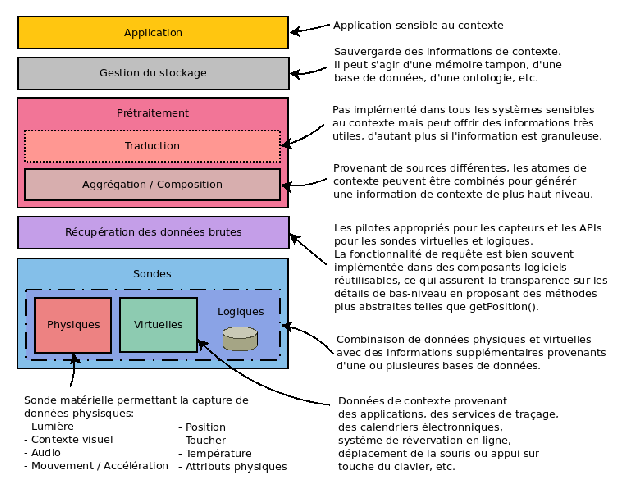
\includegraphics[width=\textwidth]{img/layered_conceptual_framework}
  \caption{Framework conceptuel d'un système sensible au contexte}
  \label{archi}
\end{figure}

\subsection{Sécurité et confidentialité}

\begin{figure}[h]
  \centering
  \begin{tabular}{l}
    La confidentialité est intrinsèquement liée au contrôle.
    \cite{ackerman_privacy_2001} \\
    \em \footnotesize Mark Ackerman, Trevor Darrell, and Daniel Weitzner. 
    Privacy in Context. \\
    \em \footnotesize Human-Computer Interaction, 16(2):167–176, December 2001.
    \\
  \end{tabular}
  \caption{La confidentialité par Ackerman}
  \label{fig:quote}
\end{figure}


Comme le contexte est susceptible de contenir des informations sensible sur des
personnes, leur situation géographique ou leur activité par example, il est
nécéssaire de protéger le caractère personnel de ces données. Les systèmes
sensibles au contexte soulèvent des défis en termes de confidentialité
inhabituels et inconsidérés par les systèmes traditionnels. La question quant au
contrôle des différents capteurs et services n'est pas abordée dans Dey et al.
\cite{dey_conceptual_2001}, et bien souvent, des applications telles que le
Context Toolkit sont supposées être sous le contrôle d'un ''utilisateur''. Les
utilistateurs sont assignés comme propriétaires des données sondées par leurs
soins. Ils sont par ailleurs autorisés à octroyer l'accès à ces données à
d'autres utilisateurs.

Néamoins, en ce qui concernent les sondes capables de déterminer la présence
d'individus dans une pièce ou à tout autre endroit, il n'existe aucunes
préconisations à ce sujet. C'est un point toutefois critique.

D'une manière générale, dans une environemment mettant à
disposition un certain eventail d'applications sensibles au contexte, un individu opère
à travers de mutliples environnemments sociaux, qui eux même font l'usage des
données d'un grand nombre d'autres individus.

epackage{float}
Aspects souvent négligés, la sécurité et la confidentialité font partie des
composantes les plus importantes d'un système sensible au contexte, car la
protection des données sensibles doit être garantie.

\section{Systèmes et frameworks existants}



\subsection{Technologies de détection}

\subsection{Représentations du contexte}

\subsection{Découverte des ressouces}

\subsection{Gestion du contexte historique}

\subsection{Sécurité et confidentialité}

\subsection{Conclusion}

% \begin{figure}
% \begin{verbatim}
% #include <iostream>
% int main(int argc, char** argv) {
%   std::cout << "Hello World." << std::endl;
%   return 0;
% }
% \end{verbatim}
%   \caption{Example source code.}
%   \label{fig:sourcecode}
% \end{figure}

%%% Local Variables: ***
%%% mode: latex ***
%%% TeX-master: "thesis.tex" ***
%%% End: ***

\chapter{Problématiques émergentes \newline et orientations de recherche}

Dans ce mémoire, nous avons décrit divers modèles et principes de conception
d'un système sensible au contexte et présenté une multitude d'intergiciels et
d'approches distribuées pour simplifier la configuration d'applications
sensibles au contexte. De cet état de l'art se dégagent plusieurs problématiques
dans le développement d'un système de configuration basé sur le contexte
auxquelles nous tenterons d'apporter une solution.

\section{Intergiciel et détails d'implémentation}

Le besoin d'un nouvel intergiciel se fait ressentir du coté de l'implémentation.
Les technologies intergicielles actuelles ne sont pas adaptées pour le prise en
considération des restrictions imposées pas la mobilité et les systèmes
environnementaux intelligents : connexions volatiles, traitements et restrictions
mémoire sur les périphériques mobiles, canaux de communication étroits, écrans
réduits, mécanismes d'entrées restreintes, et la liste continue. Il existe
néanmoins une gamme d'implémentations de systèmes sensible au contexte dans la
littérature avec quelques prototypes fonctionnels :

\begin{itemize}
    \item \textbf{Hydrogen} \cite{hofer_context-awareness_2003}: 
        une architecture en trois couches.
    \item \textbf{Gaia} \cite{chetan_mobile_2005}: 
        une autre infrastructure intergicielle, étends les caractéristiques
        génériques des systèmes d'exploitation pour y incorporer la
        sensibilité au contexte.
    \item \textbf{CybreMinder} \cite{abowd_context-aware_2002}: 
        un système sensible au contexte permettant de générer des messages
        de rappel.
    \item \textbf{Context Toolkit} \cite{dey_conceptual_2001}: 
	    une architecture basée sur les widgets.
\end{itemize}

\section{Représentation des informations de contexte}

L'une des principales innovations à apporter dans les infrastructures
d'applications sensibles au contexte réside dans l'introduction d'une interface
présentant un niveau d'abstraction élevé. Cela permettrait de représenter la
connectivité des composants applicatifs avec les politiques de haut niveau qui
la régissent.Cette couche doit rester simple d'utilisation pour les
développeurs d'applications, et le modèle améliorer simultanément
l'automatisation et la sécurité.

\subsection{Ontologie de contexte}

La représentation des informations de contexte est grande préoccupation. Nous
avons présenté dans ce mémoire une approche basée sur les ontologie très
générique. Elle est basée sur quatre concepts fondamentaux : utilisateur,
environnement, plateforme et ressources. Actuellement, les ontologies sont
surtout utilisées pour permettre la communication entre les différents
périphériques dans le même réseau. Comme proposé par le ContextUML
\cite{sheng_contextuml:_2005}, le Langage de Modélisation Unifié (UML) peut
également être utilisé pour modéliser le contexte. Ces modèles pourraient être
utilisés pour séparer la définition et l'information liée au contexte de
l'implémentation spécifique. Il existe d'autres caractéristiques qui font que
l'information de contexte est difficile à modéliser : comme abordé précédemment,
il est parfois nécessaire de différencier une information statique d'une
information dynamique.

\subsubsection{Ontologie de services}

\begin{itemize}
  \item ServiceProfile (partie ''Quoi'')
  \item ServiceModel (partie ''Comment abstrait'')
  \item ServiceGrounding (partie ''Comment concret'')
\end{itemize}

Tout comme pour la standardisation de la gestion intelligente de la
configuration, la classe ServiceModel est très importante. Les services sont
modélisés comme des processus et la classe Process est utilisée pour indiquer
les opérations à des niveaux granularité différents. La classe Process comprend
principalement deux types de processus : atomiques et composites. Puisque
l'information de gestion de configuration est définie comme un ontologie OWL,
l'information peut être utilisée comme les paramètres des opérations de gestion
de la configuration, qui sont définis sous la forme de processus composites.
Chaque service de gestion de configuration correspond à un processus composite,
lui-même composé de plusieurs processus atomiques. Quand le gestionnaire invoque
un service de gestion de configuration prédéfini en OWL-S, le service sera alors
exécuté pour le dispositif réseau en place.

\section{Règles sémantiques et politiques de comportement}

Un autre domaine de recherche concernerait l'utilisation de règles pour exprimer
les comportements souhaités en termes d'éléments de haut niveau. Des langages
de définition de règles sont utilisés dans certains cas pour obtenir la
sensibilité au contexte. CRIME \cite{murphy_coordination_2007} par exemple, est
une implémentation prototypique du modèle Fact Space, qui est un langage de
coordination fournissant aux applications une vue de leur environnement. Les
règles CRIME décrivent le comportement des applications conformément à
l'information de contexte. CRIME traite également les déconnexions en invalidant
les faits et conclusions qui sont tirés des périphériques qui ne sont plus
disponibles dans l'environnement.

\subsection{Gestion basée sur des politiques (Policy-Based)}

La politique est identifiée comme une spécification de la configuration moyenne
du système sur des périodes persistantes. Un aspect important de cette
définition est qu'elle permet une certaine tolérance à l'erreur, nécessitée par
les évènements aléatoires se produisant susceptibles de corrompre la politique
en place dans la boucle de gestion du système. Il existe un élément probabiliste
ou stochastique pour le comportement du système et, par conséquent, la politique
ne peut être qu'une propriété moyenne en général.

\subsection{Modèle de définition des politiques d'administration}

Le modèle permettant la définition des politiques d'administration serait un
modèle orienté sur les ontologies et basé sur la théorie de la promesse.
Celle-ci s'appuie sur un contrôle évolutif des objets intelligents,
contrairement aux modèles impératifs plus traditionnels pensés comme des
systèmes de gestion descendants. Dans ces derniers, le gestionnaire central
doit être informé des commandes de configuration des objets sous-jacents et de
l'état actuel de ces objets.

Au sein du contexte, le modèle fournit une série d'objets qui définissent
l'application. Les objets englobent les terminaux, les groupes de terminaux et
les politiques qui définissent leurs relations.

L'infrastructure conçoit un modèle d'objet pour le déploiement d'applications,
ces dernières constituant le point central. Historiquement, les applications
étaient limitées par les capacités du réseau et par des configurations visant à
prévenir leur utilisation abusive. Des concepts tels que l'adressage, le VLAN et
la sécurité sont depuis toujours intrinsèquement liés, ce qui limite
l'évolutivité et la mobilité des applications. Alors que les applications sont
redessinées pour la mobilité et l'évolutivité web, cette approche traditionnelle
empêche leur déploiement rapide et homogène.

\subsection{Théorie de la promesse}

La théorie de la promesse est une théorie nouvelle sur ce qu'il peut arriver
dans un réseau de composants entièrement autonomes.

Plutôt que d'adopter la croyance conventionnelle que ''seulement ce qui est
programmé peut arriver'', elle pren le point de vue opposé : ''seulement ce
qui est promis peut être prédit''. Elle aborde donc la gestion du point de vue
de l'incertitude avec réalisme plutôt que celui de la foi en la conformité. Dans
la théorie de la promesse, on suppose un point de vue orienté service des
interactions entre les différents dispositifs informatiques. Chaque nœud propose
de jouer un rôle dans un réseau de collaboration en promettant de restreindre
son comportement de différentes manières. Une utilisation typique de la théorie
de la promesse est d'examiner le comportement en régime permanent d'un certain
nombre d'agents (composants) autonomes. La théorie de la promesse ne détermine
pas nécessairement pleinement le comportement de ses composants, elle représente
seulement les contraintes au sein d'un ensemble de comportements définis. Elle
n'est pas limitée aux promesses linéaires.

La théorie de la promesse adhère à un point de vue orienté service des
politiques des gestion et utilise un langage graphique pour composer et analyser
les propriétés systèmes.

Une caractéristique essentielle des promesses est qu'elles séparent clairement
ce qui contraint et à qui la contrainte s'applique. C'est un autre domaine qui
soulève bien souvent des confusions dans la théorie des politiques. Néanmoins,
le modèle ontologique permet un fois de plus de bien distinguer ces deux
aspects grâce à son haut degré de formalisme.

\subsubsection{CfEngine3: une implémentation de référence de la théorie de la
promesse}

CfEngine3 implémente deux approches :

\begin{itemize}
    \item \textbf{Centralisée}: 
        le système va pousser avec force les règles et règlements établis de
        manière centralisée avec ou sans la volonté de l'utilisateur final hôte.
    \item \textbf{Basé sur des politiques} :
        cette approche fonctionne de la même manière que le protocole SNMP
        (Simple Network Management Protocol), à l'exception qu'elle donne une
        autonomie totale aux agent, de manière à ce qu'ils aient plein droit de
        tirer et implémenter un ensemble centralisé de politiques de
        configuration.
\end{itemize}

En théorie, chacun des agents autonomes va faire formuler une promesse sur le
comportement qu'on attend de lui, basé sur un choix qui lui est propre. C'est ce
que rend la théorie de la promesse optimale pour un framework de gestion basé
sur des politiques.

La théorie de la promesse décrit des services régies par des politiques, dans un
framework d'agents complètement autonomes, qui s'aident les uns les autres
seulement par une coopération volontaire. Dans CfEngine3, chaque élément de
configuration va faire une promesse concernant ses caractéristiques propres et
sa relation avec d'autres éléments de configuration.

Nous souhaitons être en mesure de promettre que le système est cohérent, de le
vérifier et d'effectuer des changements seulement si nos promesses ne sont pas
tenues. Cela nécessite, en plus de l'implémentation initiale de ces promesses,
la vérification continue de l'état de chacun des éléments de configuration
vis-à-vis de leur promesses respectives pour assurer un système cohérent et en
conformité avec les politiques en vigueur.

% TODO : expliquer ITIL
%Pour comprendre ITIL (Information Technology Infrastructure Library), il
%faut l'imaginer comme un service fourni par CfEngine.

\subsubsection{Définition de la promesse}

Une promesse est différente d'un engagement : un engagement est le moment où un
agent rompt avec une ligne de conduite pour une autre discontinue avec des vues
sur un objectif, la plupart du temps à travers une action spécifique ou un
investissement sur des résultats futurs. Dans certains cas, l'acte
d'engagement peut résulter en une promesse persistante, mais promettre
n'implique pas une action provoquant un changement discontinu.

\begin{figure}[H]
    \centering
    \begin{tabular}{l}
        ``Une promesse est la spécification d'un état ou comportement \\
        ultérieur d'un agent autonome à un autre. Elle est ainsi, \\
        une unité de politique.`` \cite{burgess_modeling_2006} \\
        \em \footnotesize Mark Burgess, Alva Couch, Modeling Next Generation
        Configuration Management Tools, \\
        \em \footnotesize Pp. 131-147 of the Proceedings of LISA '06,
        Décembre 2006
    \end{tabular}
    \caption{La promesse par Burgess et al. (2006)}
    \label{fig:quote}
\end{figure}

Les promesses sont faites à un agent par un agent et sont modélisées par une
relation unidirectionnelle labellisée par un \emph{corps} de promesse qui
définit la substance de la promesse. Une promesse avec le \emph{corps}
\textbf{+b} est une déclaration pour ''donner'' un comportement d'un agent à un
autre, tandis qu'une promesse avec le \emph{corps} \textbf{-b} est la
spécification de quel comportement sera reçu, accepté ou utilisé d'un agent à
l'autre.

\subsubsection{Caractéristiques de la promesse}

Un promesse est l'annonce d'un fait ou d'un comportement d'un prometteur à un
promis, sous le regard d'un certain nombre de témoins (définissant le champ
d'application de la promesse), dont le résultat n'a pas encore été évalué.  On
distingue deux types de promesses :

\begin{itemize}
    \item Une promesse d'accepter de se comporter comme une autre. C'est
        essentiel pour la définition de groupes, de rôles ou de structures
        sociales avec un consensus de comportement (cf.
        section~\ref{sec:consensus})
    \item Une promesse d'utiliser la promesse d'un autre. C'est crucial pour les
        interactions client/serveur, les dépendances et les contrôles d'accès.
\end{itemize}

Un promesse présentes les caractéristiques suivantes :

\begin{enumerate}
    \item Il doit y avoir des agents pour qu'une promesse existe.
    \item Il doit y avoir un prometteur (ou agent source).
    \item Il doit y avoir un promis (ou agent destinataire), qui peut très bien
        aussi être la source.
    \item Il doit y avoir un \emph{corps} qui décrit la nature de la promesse.
\end{enumerate}

\subsubsection{Représentation et types de promesse: $\pi$-calculus}

\begin{table}[H]
    \begin{tabularx}{\textwidth}{
            >{\centering\arraybackslash}X|
            >{\centering\arraybackslash}X|
            >{\centering\arraybackslash}X|
        }

        \cline{2-3}
        & 
        \textbf{Notation} &
        \textbf{Interprétation} \\ 

        \cline{2-3}
        &
        $a \xrightarrow{+b} a'$ &
        Promesse avec le \emph{corps} $b$ \\

        &
        $a' \xrightarrow{-b} a$ &
        Promesse d'accepter $b$ \\

        &
        $v_a(a \xrightarrow{b} a')$ &
        La valeur de la promesse à $a$ \\

        \cline{1-1}
        \multicolumn{1}{ |X| }{\textbf{Type de promesse}} &
        $v_{a'}(a \xrightarrow{b} a')$ &
        La valeur de la promesse à $a'$ \\

        \cline{1-3}
        \multicolumn{1}{ |c| }{Basique} &
        $n_1 \xrightarrow{\pi} n_2$ &
        Fournit un service / un flux \\

        \multicolumn{1}{ |c| }{Coopérative} &
        $n_1 \xrightarrow{C(\pi)} n_2$ &
        Imite / Suit \\

        \multicolumn{1}{ |c| }{Utilisatrice} &
        $n_1 \xrightarrow{U(\pi)} n_2$ &
        Utilise / Accepte de la part de\\

        \multicolumn{1}{ |c| }{Conditionnelle} &
        $n_1 \xrightarrow{\pi_1/\pi_2} n_2$ &
        ``File`` de promesses: $\pi_1$ if $\pi_2$\\
        \cline{1-3}
    \end{tabularx}
    \caption{Représentation et types de promesses}
    \label{PromiseTypes}
\end{table}
   
Les promesses de services basiques forment un certain nombre de types, comme par
exemple `fournir un web service en moins de 5 millisecondes` ou `donner
n'importe quel information sur l'agent X`. D'autres exemples :

\begin{itemize}
    \item $X \xrightarrow{q \leq q_0} Y $: l'agent $X$ promet de ne jamais éxeder la
        limite $q \leq q_0$.
    \item $X \xrightarrow{q = q_0} Y $: l'agent $X$ promet de satisfaire
        $q = q_0$.
    \item $X \xrightarrow{\ell \subseteq  L} Y $: $X$ promet de garder $\ell$
        comme sous-langage du langage L
    \item $X \xrightarrow{S} Y $: $X$ offre le service $S$ à $Y$.
    \item $X \xrightarrow{R} Y $: $X$ promet de relayer $R$ à $Y$.
    \item $X \xrightarrow{\neg R} Y $: $X$ promet de ne jamais relayer $R$ à $Y$.
    \item $X \xrightarrow{S,t} Y $: $X$ promet de répondre avec le service $S$
        en l'espace de $t$ secondes.
\end{itemize}

Une promesse est dite ``rompue`` si un agent fait deux promesses différentes du
même type en même temps (différent d'une promesse qui aurait expiré ou changé).

\subsubsection{Processus de raisonnement lié à la promesse}

Le procédé de raisonnement qui accompagne l'émanation d'un promesse, se divisent
en plusieurs sous-étapes, accrochez-vous:

\begin{itemize}
  \small
  \item \textbf{Préparation de la promesse} :
	Processus de raisonnement effectué par A conduisant à la conception, la
	synchronisation et la délivrance de la promesse P par A.
  \item \textbf{Analyse de crédibilité} :
	Processus de raisonnement où les agents C dans le champ d'application de
	la promesse P déterminent la crédibilité qu'ils assignent à A promettant
	P compte tenu des faits connus de A (mais à l'exception des informations
	historiques précises sur le comportement individuel d'un membre de sa
	classe d'agent)
  \item \textbf{Détermination préliminaire de la confiance} :
	Processus de raisonnement effectué par C (C dans le domaine
	d'application de la promesse P) servant à :
  	\begin{enumerate}
	  \item Déterminer la confiance que C accorde à A avant même de
		  connaitre la promesse P (confiance préalable)
	  \item Spécifier quelles sont les attentes générées par la prise en
		  considération de la promesse P.
  	\end{enumerate}
  \item \textbf{Délibération de contre-promesse} :
	Processus de raisonnement effectué par B concernant les contre-promesses
	pouvant potentiellement être émises par B en retour de considération de
	P (B dans le champ d'application de P)
  \item \textbf{Prédiction de l'impact de la promesse} :
	(cela peut être réalisé à condition que B ait émis une ou plusieurs
	contre-promesses plausibles)
  	\begin{enumerate}
	  \item Processus de raisonnement effectué par B (dans le champ
		  d'application de P) et C (n'importe quel agent dans le champ
		  d'application de P) servant à déterminer les (le changement
		  des) attentes que P créé dans B (et que A a l'intention de
		  générer).  
	  \item Processus de raisonnement visant à la modification des ententes
		  (détenues par B ou C) étant donné la changement des attentes
		  de chacun d'entre eux amené par la prise en considération de
		  la promesse P.
  	\end{enumerate}
  \item \textbf{Évaluation de la promesse} :
	Processus de raisonnement effectué par C concernant :
  	\begin{enumerate}
	  \item La façon dont C va évaluer si la promesse de A a été tenue ou
		  non.
      \item L'évaluation de cette dernière au moyen de la méthode la plus
          adéquate
  	\end{enumerate}
  \item \textbf{Surveillance de rétraction de promesse} :
	A peut être amené à un stade ultérieur à émettre une autre promesse Q,
	pour laquelle la tenue n'est pas compatible avec la tenue de P. Dans ce
	cas, Q qualifie un retrait de P. Un agent C applique un processus de
	raisonnement qui surveille et évalue les promesses postérieures émises
	par A pour déterminer si celles-ci seront amenées à rompre la promesse P
	et induire sont retrait.
  \item \textbf{Mise à jour de la confiance} :
	Processus de raisonnement en place pour chacun des agents C dans le champ
	d'application de P visant à mettre à jour la confiance préalablement
	accordée à A, en adéquation avec la résultat de l'évaluation que C fait
	concernant le degré avec lequel la promesse P a été tenue par A.
  \item \textbf{Critère de réputation} :
	Processus de raisonnement effectué par chacun des agents C dans le champ
	d'application de P visant à échanger entre les différent agents les
	effets des mises à jour de confiance. Le flux de réputation permet a un
	agent C n'ayant aucuns aprioris sur un agent A d'acquérir une confiance
	initiale en prenant en considération les preuves recueillies par les
    autres agents (parce que même les agents ont des casiers judiciaires).
\end{itemize}

\subsection{Gestion de configuration basée sur la théorie de la promesse}

\subsubsection{Données paramètres}

Un système de gestion de configuration basé sur la théorie de la promesse
accepte comme paramètres d'entrée un ensemble de politiques de configuration de
haut niveau. Ces politiques de haut niveau seront divisées en spécifications de
configuration de bas niveau, que nous appellerons ``promesses`` dans la
modélisation par la théorie de la promesse. Notre ontologie permettra
formalisation de ces promesses.

En complément des politiques de configuration, les informations suivantes
pourront être transmises au système de gestion de configuration :

\begin{itemize}
    \item Le nombre et le type de machines nécessaires
    \item Le système d'exploitation de chacune des machines
    \item Les paquets ayant besoin d'être installés sur chaque machine
    \item Les services que chacun des hôtes doit fournir
    \item Les préoccupations liées au stockage comme le type de système de
        fichiers
    \item Les questions de sécurité, incluant notamment les aspect de gestion
        des utilisateurs
\end{itemize}

\subsubsection{Traitements}

Les politiques de configuration de haut niveau subirons deux traitements majeurs
:

\begin{enumerate}
    \item Spécification de la configuration de bas niveau. Ce traitement dépend
        de l'information liée à l'architecture telle que le détail du
        périphérique ou le type de topologie attendu par un système.
    \item Respecter les promesses formulées par chacun des éléments de
        configuration. Ce traitement consiste à ce que chaque élément de
        configuration se comporte conformément à leurs promesses. Dans la
        gestion des changements, CfEngine3 prendra des mesures correctives en
        plus de jouer le rôle d'informer les parties concernées en cas de non
        tenue d'une promesse.
\end{enumerate}

\subsubsection{Résultats attendus}

Le résultat de ces traitements est un système conforme aux règles politiques en
vigueur où chaque élément de configuration possèdent les clés et valeurs
attendues.  Autrement dit, un ensemble d'ordinateurs avec les valeurs de
configuration appropriées (les valeurs d'attribut promises).  Les éléments de
configuration principaux sont les fichiers, les paquets, les disques, les
processus, le services et les interfaces. 

En plus de leurs propres valeurs d'attributs et manière d'agir, un ensemble de
promesses sur le bon type de relations entre ces éléments de configuration est
nécéssaire pour valider le résultat de ces traitements.

\section{Consistance de l'information et tolérance à l'échec}

\subsection{Algorithme de consensus}
\label{sec:consensus}

Le consensus est un problème fondamental dans les systèmes distribués tolérants
aux pannes. Un consensus implique de multiples serveurs acceptant des valeurs.
Une fois qu'ils atteignent une décision sur une valeur, cette décision est
définitive. Les algorithmes de consensus typiques sont amenés à faire des
progrès lorsque la majorité de leurs serveurs sont disponibles, par exemple, un
cluster de 5 serveurs peut continuer à fonctionner même si deux serveurs ne sont
plus disponibles. Si plusieurs serveurs échouent, ils cessent de faire des
progrès (mais ils ne retournerons jamais de valeurs erronées).

\subsubsection{Pourquoi Raft ?}

Raft est un algorithme de consensus qui est conçu pour être facile à comprendre.
Il est équivalent à Paxos dans la tolérance aux pannes et en termes de
performance. La différence est qu'il est décomposé en sous-problèmes
relativement disjoints, et traite de manière rigoureuse toutes les pièces
majeures nécessaires pour obtenir un système cohérent.

Il existe des écarts significatifs entre la description de l'algorithme de Paxos
et les besoins d'un système dans le monde réel. Le système au final serait basé
sur un protocole dénué de preuves.

\begin{tabular}{p{.48\textwidth}p{.48\textwidth}}
    \noindent
    \textbf{\textit{Inconvénients de Paxos}}
    \small

    \begin{itemize}
        \item Extrêmement difficile à comprendre. L'opacité de Paxos dérive de
            son choix d'avoir un sous-ensemble de décrets uniques comme son
            fondement.
        \item Ne fourni pas une bonne base pour la construction d'applications
            pratiques. Par exemple, il y peu d'avantages à choisir de manière
            indépendante une collection d'entrées dans le registre, pour les
            fusionner par la suite dans un journal séquentiel ; cela ajoute
            juste de la complexité. Il est plus simple et plus efficace de
            concevoir un système autour d'un journal, où les nouvelles entrées
            sont ajoutées séquentiellement dans un ordre contraint.
        \item Utilise une approche symétrique pair-à-pair à sa base. Cela a un
            sens dans un monde simplifié où seule une décision sera prise, mais
            peu de systèmes concrets utilisent cette approche.  Si une série de
            décisions doivent être prises, il est plus simple et plus rapide
            d'élire d'abord un leader, puis de le laisser coordonner les
            décisions.
    \end{itemize} 
    
    &

    \textbf{\textit{Avantages de Raft}}
    \small

    \begin{itemize}
        \item Raft utilise une forme plus solide de leadership que les autres
            algorithmes de consensus. Par exemple, les entrées du registre de
            seront communiquées que par le leader vers les autres serveurs. Cela
            simplifie largement la gestion de la réplication des journaux et
            rend Raft beaucoup plus facile à comprendre.
        \item Raft utilise des minuteries aléatoires pour élire les leaders.
            Cela ajoute un peu de mécanismes au système de pulsation déjà
            nécessaire dans n'importe quel algorithme de consensus, tandis que
            la résolution des confits se fait simplement et rapidement.
        \item Le mécanisme de Raft pour changer l'ensemble des serveurs de la
            grappe utilise une nouvelle approche de consensus conjointe où les
            majorités des deux différentes configurations se superposent pendant
            les transitions. Cela permet au groupe de continuer à fonctionner
            normalement pendant les changements de configuration.
    \end{itemize}

\end{tabular}

\subsubsection{Architecture de machines à états répliquées}

\begin{wrapfigure}[8]{r}[0pt]{.4\textwidth}
    \centerline{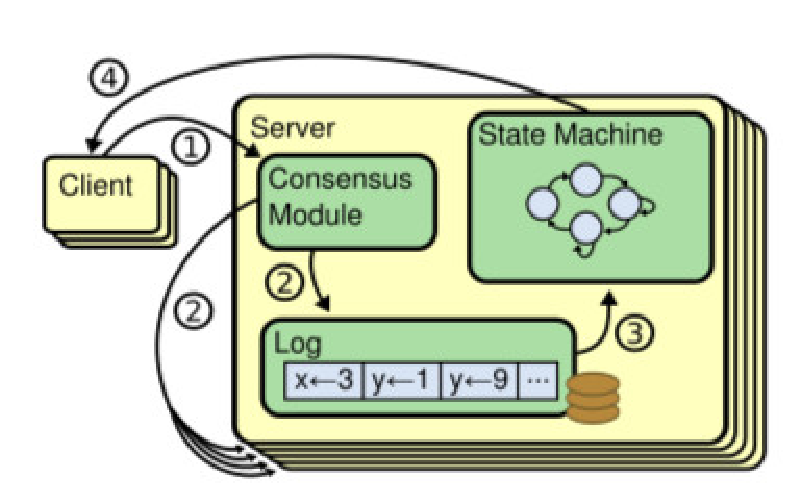
\includegraphics[width=.37\textwidth]{img/replicated_state_machine}}
    \caption{Procédé de réplication des machines à états}
    \label{replicated_state_machine}
\end{wrapfigure}

L'algorithme de consensus gère un registre répliqué contenant les commandes de
la machine à états de chacun des clients dans le réseau. Les machines à états
traitent des séquences identiques de commandes à partir de journaux partagés, de
sorte qu'ils produisent les mêmes résultats.

Les systèmes à grande échelle n'ayant qu'un seul cluster leader utilisent une
machine à état distincte pour gérer les élections et pour stocker les
informations de configuration qui doivent survivre aux crashs du leader
(exemple: Chubby, ZooKeeper).

\begin{verse}
    \underline{
        Garder le registre répliqué consistant est le travail de l'algorithme de
        consensus.
    }
\end{verse}

Les algorithmes de consensus pour les systèmes concrets ont généralement les
caractéristiques suivantes :

\begin{itemize}
    \item Ils assurent la sécurité (ne retournent jamais de résultat erroné)
        sous toutes conditions non byzantines, y compris les retards dans le
        réseau, les pertes de partitions et de paquets, la duplication et
        la réorganisation.
    \item Ils sont entièrement fonctionnels (disponibles) dans la mesure où au
        moins la majorité des serveurs sont opérationnels et peuvent communiquer
        les uns avec les autres et avec les clients. Ainsi, un groupe type de
        cinq serveurs peut tolérer la défaillance de deux ses membres. Les
        serveurs sont supposés tomber en panne en s'arrêtant ; ils pourront plus
        tard retrouver un état stable et rejoindre le cluster.
    \item Il ne dépendent pas de la contrainte temporelle pour assurer la
        cohérence des journaux : des horloges défectueuses et des retards
        abusifs dans la délivrance des messages peuvent causer des problèmes de
        disponibilité. 
    \item Dans le cas le plus courant, une commande peut s'achever aussitôt que
        la majorité de la grappe a répondu à un seul tour d'appels à procédures
        distantes ; une minorité de serveurs lents de doivent pas impacter les
        performances globales du système.
\end{itemize}

\subsubsection{États des serveurs}

\begin{wrapfigure}[7]{r}{.4\textwidth}
    \vspace{-12pt}
    \centerline{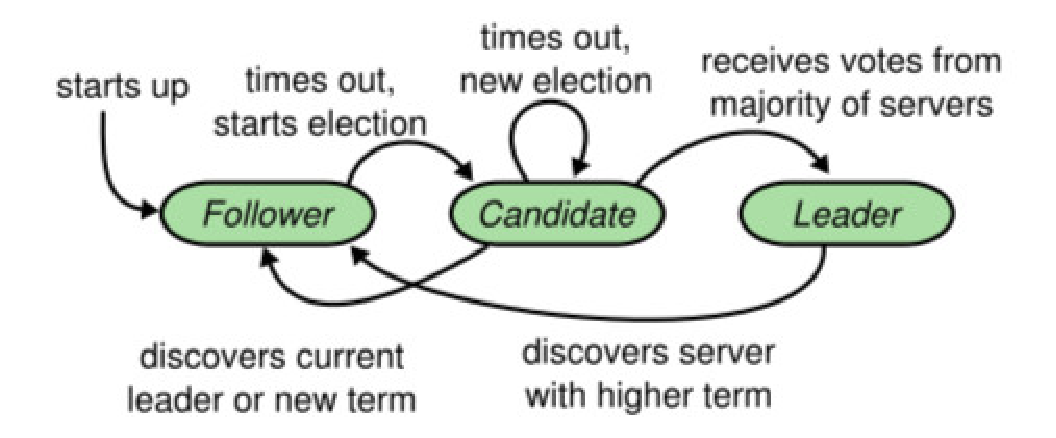
\includegraphics[width=.37\textwidth]{img/raft_server_states}}
    \caption{États et transitions dans un cluster Raft}
    \label{fig:raft_server_states}
    \vspace{12pt}
\end{wrapfigure}

Un cluster Raft comprend une multitude des serveurs (cinq est un nombre courant
permettant au système de tolérer deux échecs). À n'importe quel moment donné,
chacun des serveur est dans l'un de ces états :

\begin{itemize}
    \item \textbf{Leader} :
        En cycle normal, il existe un et un seul \emph{leader} et tous les autres
        serveurs sont \emph{followers}. Le \emph{leader} traite les requêtes de
        tous les clients (si un client contacte un \emph{follower}, le
        \emph{follower} le redirige vers le \emph{leader}).
    \item \textbf{Follower} :
        Les \emph{followers} sont passifs : ils n'émettent jamais de messages par
        leur propre initiative, ils se contentent simplement de répondre aux
        requêtes émises par le \emph{leader} et les \emph{candidats}.
    \item \textbf{Candidat} :
        Statut intermédiaire utilisé lors de l'élection d'un nouveau
        \emph{leader}. La figure \ref{fig:raft_server_states} montre les différents états
        et transitions possibles dans le consensus de Raft.
\end{itemize}

Les \emph{followers} ne font que répondre aux requêtes des autres serveurs. Si
un \emph{follower} ne reçoit plus de communications, il devient alors
\emph{candidat} et initie une élection. Le \emph{candidat} qui reçoit les votes
d'un majorité du cluster complet devient le nouveau \emph{leader}. D'une manière
générale, les \emph{leaders} opèrent jusqu'à ce qu'ils échouent.

\subsubsection{Élection d'un \emph{leader}}

\begin{wrapfigure}{r}{.4\textwidth}
    \centerline{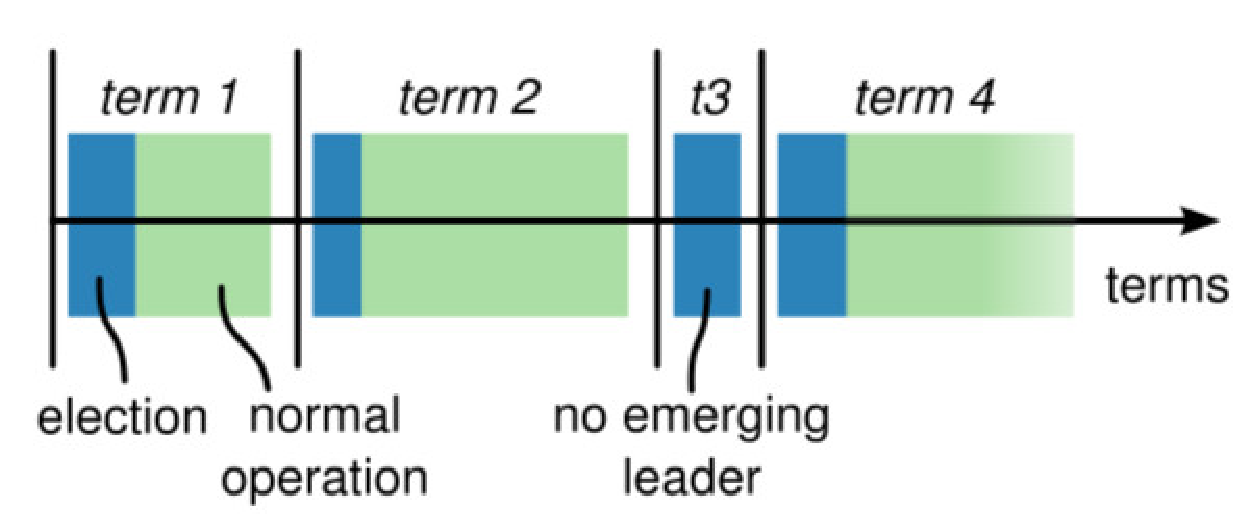
\includegraphics[width=.37\textwidth]{img/leader_election}}
    \caption{Processus d'élection d'un \emph{leader}}
    \label{fig:leader_election}
\end{wrapfigure}

Comme le montre la figure \ref{fig:leader_election}, le temps est divisé en
termes. Chaque terme commence par une élection. Après une élection fructueuse,
un \emph{leader} unique gère l'intégralité du cluster jusqu'à la fin du terme.
Parfois les élections échouent, auquel cas le terme se terminera sans choisir de
\emph{leader} et de nouvelles élections auront lieu au prochain terme. Il est
important de noter que les transitions seront observées à des moments différents
d'un serveur à l'autre.

\subsubsection{Réplication des journaux}

\begin{wrapfigure}{r}{.4\textwidth}
    \centerline{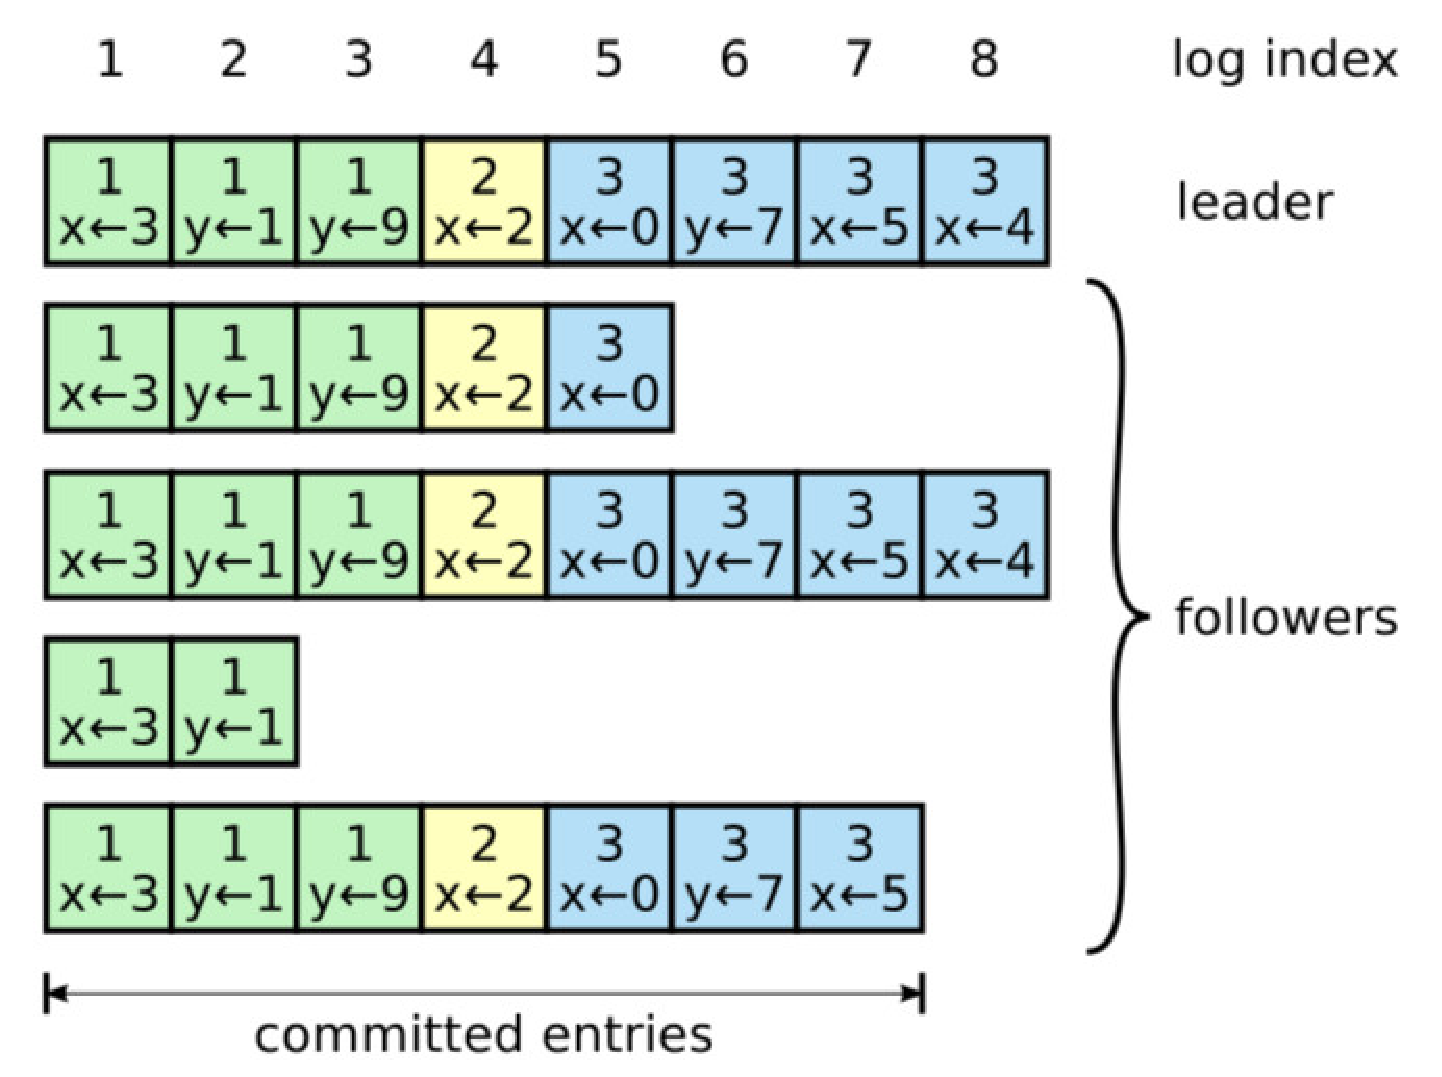
\includegraphics[width=.37\textwidth]{img/log_replication}}
    \caption{Processus de réplication des journaux}
    \label{fig:log_replication}
\end{wrapfigure}

L'organisation des journaux est détaillé par la figure
\ref{fig:log_replication}.  Les journaux sont composés d'entrées
séquentiellement numérotées. Dans notre gestionnaire de contexte, ces entrées
correspondent à des états incrémentaux de notre ontologie. Chaque entrée réfère aux terme
durant lequel elle a été créée (le numéro de case dans la figure
\ref{fig:log_replication}) et contient une commande pour la machine à état. Une
entrée est considérée comme \emph{une transaction validée (committed)} si son
insertion dans la machine à état est sans dangers.

En cycle fonctionnement normal, il y a un et un seul \emph{leader} et $n$
\emph{followers}. Le \emph{leader} envoie des pulsations régulières, témoins de
sa disponibilité, aux autres membres du cluster. Le premier \emph{follower}
remarquant l'inactivité du \emph{leader} (arrêt des pulsations) initie alors de
nouvelles élections. 

\section{Conclusion}

Les différents concepts détaillés dans ce chapitre nous permettent de répondre
aux problématiques énoncées auparavant : L'ontologie apporte le haut degré de
formalisation nécessaire pour modéliser les informations de contexte et les
promesses permettant la définition des politiques de configuration du système.
Le théorie de la promesse propose une approche sémantique de la configuration,
promettant aux utilisateurs un travail de configuration à moindres efforts.
L'algorithme de consensus garantit la tolérance à l'échec et une organisation
rigoureuse des communications inter-agents par l'attribution de rôles dans le
cluster. Le modèle de réplication des journaux qu'il implémente permet d'assurer
la permanente consistance de l'ontologie avec une simplicité remarquable.

% ex: set spelllang=fr spell: %
%%% Local Variables: ***
%%% mode: latex ***
%%% TeX-master: "thesis.tex" ***
%%% End: ***

\chapter{Simulation}


\clearpage
\phantomsection

\bibliographystyle{abbrv}
\bibliography{thesis}

\captionsetup[figure]{list=no}
\captionsetup[table]{list=no}

% The original template (from Trevor) had a custom \appendix command,
% but I found it to break figure/table counters. I'm not sure how
% reliable my fix is, so I ended up reverting back to the standard
% latex version, and renaming the custom command to \myappendix.  You
% can try both and see how things work out:
% 1) Call \appendix once, and then make each appendix a \chapter
% 2) Call \myappendix once, and then make each appendix a \section.

\appendix

%%%%%%%%%%%%%%%%%%%%%%%%%%%%%%%%%%%%%%%%%%%%%%%%%%%%%%%%%%%%%%%%%%%%%%%

\chapter{Théorie de la promesse}
\label{appendix:promise_theory}

\section{Définition de la promesse}

Une promesse est différente d'un engagement : un engagement est le moment où un
agent rompt avec une ligne de conduite pour une autre discontinue avec des vues
sur un objectif, la plupart du temps à travers une action spécifique ou un
investissement sur des résultats futurs. Dans certains cas, l'acte
d'engagement peut résulter en une promesse persistante, mais promettre
n'implique pas une action provoquant un changement discontinu.

%{%\begin{figure}[H]
%    \centering
%    \begin{tabular}{l}
        ``Une promesse est la spécification d'un état ou comportement \\
        ultérieur d'un agent autonome à un autre. Elle est ainsi, \\
        une unité de politique.`` \cite{burgess_modeling_2006} \\
        %\em \footnotesize Mark Burgess, Alva Couch, Modeling Next Generation
        %Configuration Management Tools, \\
        %\em \footnotesize Pp. 131-147 of the Proceedings of LISA '06,
        %Décembre 2006
%    \end{tabular}
    %\caption{La promesse par Burgess et al. (2006)}
    %\label{fig:quote}
%\par}%\end{figure}

Les promesses sont faites à un agent par un agent et sont modélisées par une
relation unidirectionnelle labellisée par un \emph{corps} de promesse qui
définit la substance de la promesse. Une promesse avec le \emph{corps}
\textbf{+b} est une déclaration pour ''donner'' un comportement d'un agent à un
autre, tandis qu'une promesse avec le \emph{corps} \textbf{-b} est la
spécification de quel comportement sera reçu, accepté ou utilisé.

\section{Caractéristiques de la promesse}

Un promesse est l'annonce d'un fait ou d'un comportement d'un prometteur à un
promis, sous le regard d'un certain nombre de témoins (définissant le champ
d'application de la promesse), dont le résultat n'a pas encore été évalué.  On
distingue deux types de promesses :

\begin{itemize}
    \item Une promesse d'accepter de se comporter comme une autre. C'est
        essentiel pour la définition de groupes, de rôles ou de structures
        sociales avec un consensus de comportement (cf. section
        \ref{sec:consensus})
    \item Une promesse d'utiliser la promesse d'un autre. C'est crucial pour les
        interactions client/serveur, les dépendances et les contrôles d'accès.
\end{itemize}

Un promesse présente les caractéristiques suivantes :

\begin{enumerate}
    \item Il doit y avoir des agents pour qu'une promesse existe.
    \item Il doit y avoir un prometteur (ou agent source).
    \item Il doit y avoir un promis (ou agent destinataire), qui peut très bien
        aussi être la source.
    \item Il doit y avoir un \emph{corps} qui décrit la nature de la promesse.
\end{enumerate}

\section{Représentation et types de promesse: $\pi$-calculus}

\begin{table}[H]
    \begin{tabularx}{\textwidth}{
            >{\centering\arraybackslash}X|
            >{\centering\arraybackslash}X|
            >{\centering\arraybackslash}X|
        }

        \cline{2-3}
        & 
        \textbf{Notation} &
        \textbf{Interprétation} \\ 

        \cline{2-3}
        &
        $a \xrightarrow{+b} a'$ &
        Promesse avec le \emph{corps} $b$ \\

        &
        $a' \xrightarrow{-b} a$ &
        Promesse d'accepter $b$ \\

        &
        $v_a(a \xrightarrow{b} a')$ &
        La valeur de la promesse à $a$ \\

        \cline{1-1}
        \multicolumn{1}{ |X| }{\textbf{Type de promesse}} &
        $v_{a'}(a \xrightarrow{b} a')$ &
        La valeur de la promesse à $a'$ \\

        \cline{1-3}
        \multicolumn{1}{ |c| }{Basique} &
        $n_1 \xrightarrow{\pi} n_2$ &
        Fournit un service / un flux \\

        \multicolumn{1}{ |c| }{Coopérative} &
        $n_1 \xrightarrow{C(\pi)} n_2$ &
        Imite / Suit \\

        \multicolumn{1}{ |c| }{Utilisatrice} &
        $n_1 \xrightarrow{U(\pi)} n_2$ &
        Utilise / Accepte de la part de\\

        \multicolumn{1}{ |c| }{Conditionnelle} &
        $n_1 \xrightarrow{\pi_1/\pi_2} n_2$ &
        ``File`` de promesses: $\pi_1$ if $\pi_2$\\
        \cline{1-3}
    \end{tabularx}
    \caption{Représentation et types de promesses}
    \label{PromiseTypes}
\end{table}
   
Les promesses de service basiques forment un certain nombre de types, comme par
exemple `fournir un web service en moins de 5 millisecondes` ou `donner
n'importe quel information sur l'agent X`. D'autres exemples :

\begin{itemize}
    \item $X \xrightarrow{q \leq q_0} Y $: l'agent $X$ promet de ne jamais éxeder la
        limite $q \leq q_0$.
    \item $X \xrightarrow{q = q_0} Y $: l'agent $X$ promet de satisfaire
        $q = q_0$.
    \item $X \xrightarrow{\ell \subseteq  L} Y $: $X$ promet de garder $\ell$
        comme sous-langage du langage L
    \item $X \xrightarrow{S} Y $: $X$ offre le service $S$ à $Y$.
    \item $X \xrightarrow{R} Y $: $X$ promet de relayer $R$ à $Y$.
    \item $X \xrightarrow{\neg R} Y $: $X$ promet de ne jamais relayer $R$ à $Y$.
    \item $X \xrightarrow{S,t} Y $: $X$ promet de répondre avec le service $S$
        en l'espace de $t$ secondes.
\end{itemize}

Une promesse est dite ``rompue`` si un agent fait deux promesses contradictoires du
même type et en même temps (différent d'une promesse qui aurait expiré ou changé).

\section{Processus de raisonnement lié à la promesse}

Le procédé de raisonnement qui accompagne l'émanation d'un promesse, se divisent
en plusieurs sous-étapes, accrochez-vous:

\begin{itemize}
  \item \textbf{Préparation de la promesse} -
	Processus de raisonnement effectué par A conduisant à la conception, la
	synchronisation et la délivrance de la promesse P par A.
  \item \textbf{Analyse de crédibilité} -
	Processus de raisonnement où les agents C dans le champ d'application de
	la promesse P déterminent la crédibilité qu'ils assignent à A promettant
	P compte tenu des faits connus de A (mais à l'exception des informations
	historiques précises sur le comportement individuel d'un membre de sa
	classe d'agent)
  \item \textbf{Détermination préliminaire de la confiance} -
	Processus de raisonnement effectué par C (C dans le domaine
	d'application de la promesse P) servant à :
  	\begin{enumerate}
	  \item déterminer la confiance que C accorde à A avant même de
		  connaitre la promesse P (confiance préalable)
	  \item spécifier quelles sont les attentes générées par la prise en
		  considération de la promesse P.
  	\end{enumerate}
  \item \textbf{Délibération de contre-promesse} -
	Processus de raisonnement effectué par B concernant les contre-promesses
	pouvant potentiellement être émises par B en retour de considération de
	P (B dans le champ d'application de P)
  \item \textbf{Prédiction de l'impact de la promesse} -
	(cela peut être réalisé à condition que B ait émis une ou plusieurs
	contre-promesses plausibles)
  	\begin{enumerate}
	  \item Processus de raisonnement effectué par B (dans le champ
		  d'application de P) et C (n'importe quel agent dans le champ
		  d'application de P) servant à déterminer les (le changement
		  des) attentes que P créé dans B (et que A a l'intention de
		  générer).  
	  \item Processus de raisonnement visant à la modification des ententes
		  (détenues par B ou C) étant donné la changement des attentes
		  de chacun d'entre eux amené par la prise en considération de
		  la promesse P.
  	\end{enumerate}
  \item \textbf{Évaluation de la promesse} -
	Processus de raisonnement effectué par C concernant :
  	\begin{enumerate}
	  \item la façon dont C va évaluer si la promesse de A a été tenue ou
		  non.
      \item l'évaluation de cette dernière au moyen de la méthode la plus
          adéquate
  	\end{enumerate}
  \item \textbf{Surveillance de rétraction de promesse} -
	A peut être amené à un stade ultérieur à émettre une autre promesse Q,
	pour laquelle la tenue n'est pas compatible avec la tenue de P. Dans ce
	cas, Q qualifie un retrait de P. Un agent C applique un processus de
	raisonnement qui surveille et évalue les promesses postérieures émises
	par A pour déterminer si celles-ci seront amenées à rompre la promesse P
	et induire sont retrait.
  \item \textbf{Mise à jour de la confiance} -
	Processus de raisonnement en place pour chacun des agents C dans le champ
	d'application de P visant à mettre à jour la confiance préalablement
	accordée à A, en adéquation avec la résultat de l'évaluation que C fait
	concernant le degré avec lequel la promesse P a été tenue par A.
  \item \textbf{Critère de réputation} -
	Processus de raisonnement effectué par chacun des agents C dans le champ
	d'application de P visant à échanger entre les différent agents les
	effets des mises à jour de confiance. Le flux de réputation permet a un
	agent C n'ayant aucuns aprioris sur un agent A d'acquérir une confiance
	initiale en prenant en considération les preuves recueillies par les
    autres agents (parce que même les agents ont des casiers judiciaires).
\end{itemize}

%%%%%%%%%%%%%%%%%%%%%%%%%%%%%%%%%%%%%%%%%%%%%%%%%%%%%%%%%%%%%%%%%%%%%%%

\chapter{Consensus de Raft}
\label{appendix:consensus}

\section{États des serveurs}

Un cluster Raft comprend une multitude des serveurs (cinq est un nombre courant
permettant au système de tolérer deux échecs). À n'importe quel moment donné,
chacun des serveur est dans l'un de ces états :

\begin{itemize}
    \item \textbf{Leader} -
        En cycle normal, il existe un et un seul \emph{leader} et tous les autres
        serveurs sont \emph{followers}. Le \emph{leader} traite les requêtes de
        tous les clients (si un client contacte un \emph{follower}, le
        \emph{follower} le redirige vers le \emph{leader}).
    \item \textbf{Follower} -
        Les \emph{followers} sont passifs : ils n'émettent jamais de messages par
        leur propre initiative, ils se contentent simplement de répondre aux
        requêtes émises par le \emph{leader} et les \emph{candidats}.
    \item \textbf{Candidat} -
        Statut intermédiaire utilisé lors de l'élection d'un nouveau
        \emph{leader}. La figure \ref{fig:raft_server_states} montre les différents états
        et transitions possibles dans un cluster Raft.
\end{itemize}

%\begin{wrapfigure}[7]{r}{.4\textwidth}
\begin{figure}[H]
    \centerline{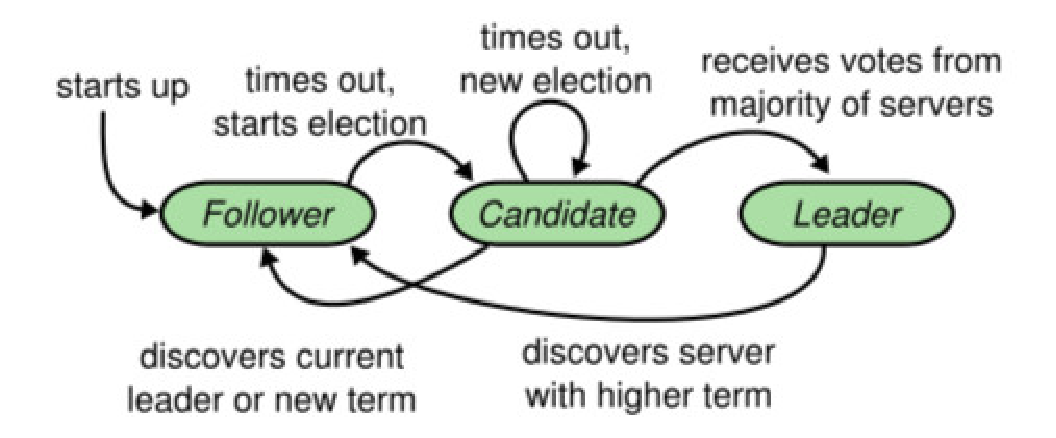
\includegraphics[width=.47\textwidth]{img/raft_server_states}}
    \caption{États et transitions dans un cluster Raft}
    \label{fig:raft_server_states}
%\end{wrapfigure}
\end{figure}

Les \emph{followers} ne font que répondre aux requêtes des autres serveurs. Si
un \emph{follower} ne reçoit plus de communications, il devient alors
\emph{candidat} et initie une élection. Le \emph{candidat} qui reçoit les votes
d'un majorité du cluster complet devient le nouveau \emph{leader}. D'une manière
générale, les \emph{leaders} opèrent jusqu'à ce qu'ils échouent.

\section{Élection d'un \emph{leader}}

Comme le montre la figure \ref{fig:leader_election}, le temps est divisé en
termes. Chaque terme commence par une élection. Après une élection fructueuse,
un \emph{leader} unique gère l'intégralité du cluster jusqu'à la fin du terme.
Parfois les élections échouent, auquel cas le terme se terminera sans choisir de
\emph{leader} et de nouvelles élections auront lieu au prochain terme. Il est
important de noter que les transitions seront observées à des moments différents
d'un serveur à l'autre.

%\begin{wrapfigure}{r}{.4\textwidth}
\begin{figure}[H]
    \centerline{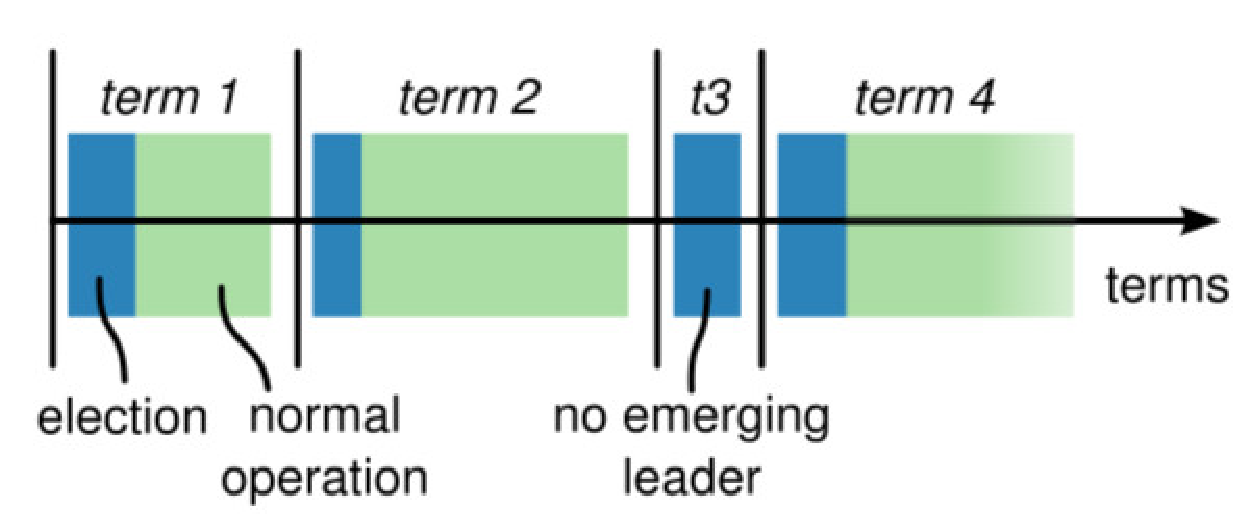
\includegraphics[width=.37\textwidth]{img/leader_election}}
    \caption{Processus d'élection d'un \emph{leader}}
    \label{fig:leader_election}
%\end{wrapfigure}
\end{figure}

\section{Réplication des journaux}

L'organisation des journaux est détaillée par la figure
\ref{fig:log_replication}.  Les journaux sont composés d'entrées
séquentiellement numérotées. Dans notre gestionnaire de contexte, ces entrées
correspondent à des états incrémentaux de notre ontologie. Chaque entrée réfère aux terme
durant lequel elle a été créée (le numéro de case dans la figure
\ref{fig:log_replication}) et contient une commande pour la machine à état. Une
entrée est considérée comme \emph{une transaction validée (committed)} si son
insertion dans la machine à état est sans dangers.

%\begin{wrapfigure}{r}{.4\textwidth}
\begin{figure}[H]
    \centerline{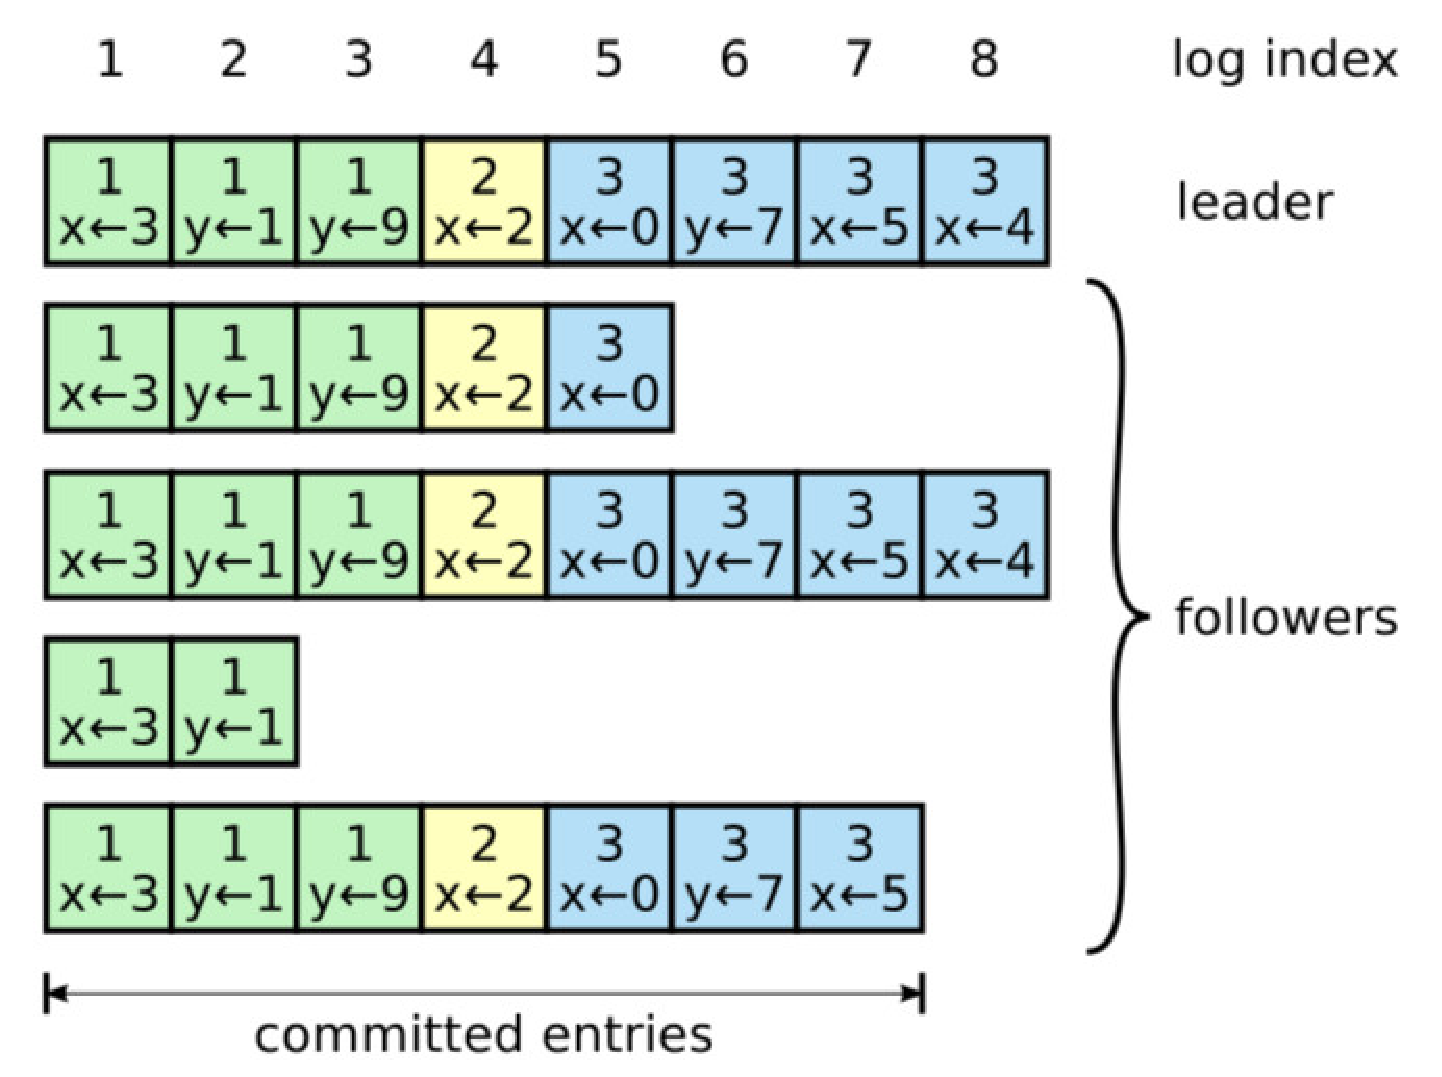
\includegraphics[width=.37\textwidth]{img/log_replication}}
    \caption{Processus de réplication des journaux}
    \label{fig:log_replication}
%\end{wrapfigure}
\end{figure}

En cycle fonctionnement normal, il y a un et un seul \emph{leader} et $n$
\emph{followers}. Le \emph{leader} envoie des pulsations régulières, témoins de
sa disponibilité, aux autres membres du cluster. Le premier \emph{follower}
remarquant l'inactivité du \emph{leader} (arrêt des pulsations) initie alors de
nouvelles élections. 

%%%%%%%%%%%%%%%%%%%%%%%%%%%%%%%%%%%%%%%%%%%%%%%%%%%%%%%%%%%%%%%%%%%%%%%

\chapter{Interface d'administration}
\label{appendix:interface}

\section{Interface pour les définition des variables de configuration de bas
niveau}
\label{appendix:interface_genconfig}

\begin{figure}[H]
    \centerline{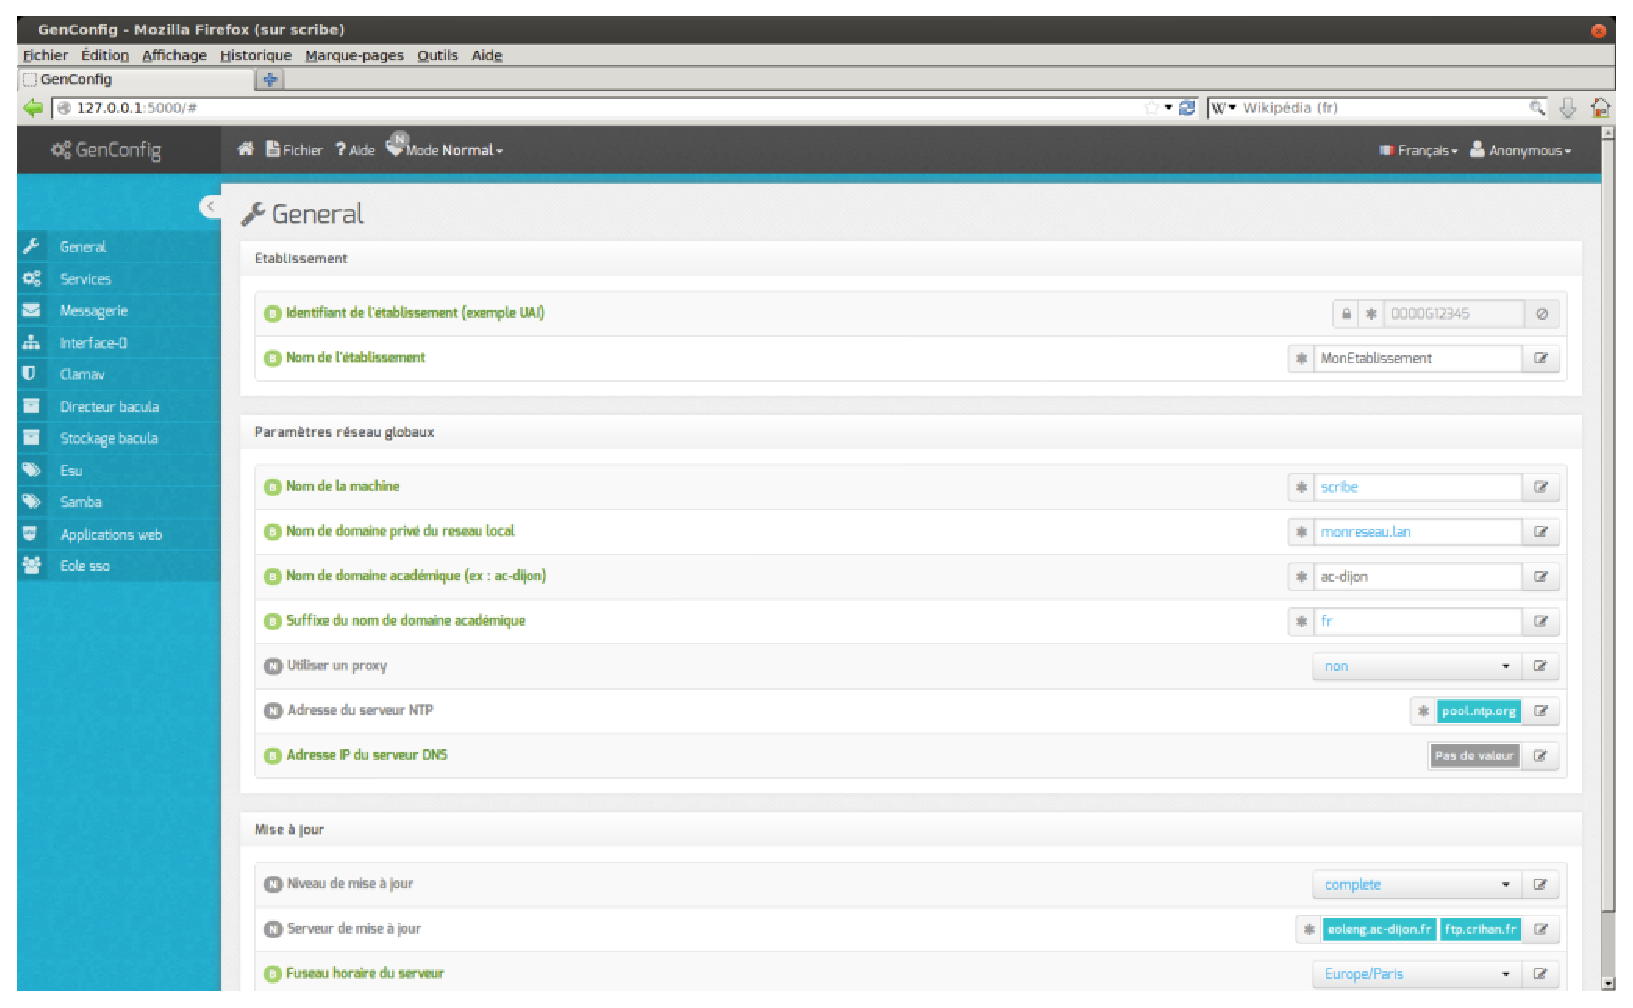
\includegraphics[width=\textwidth]{img/gen_config}}
    \caption{Interface d'administration du gestionnaire de configuration}
    \label{fig:gen_config}
\end{figure}

\section{Interface pour la consultation de l'ontologie}
\label{appendix:interface_query}

\begin{figure}[H]
    \centerline{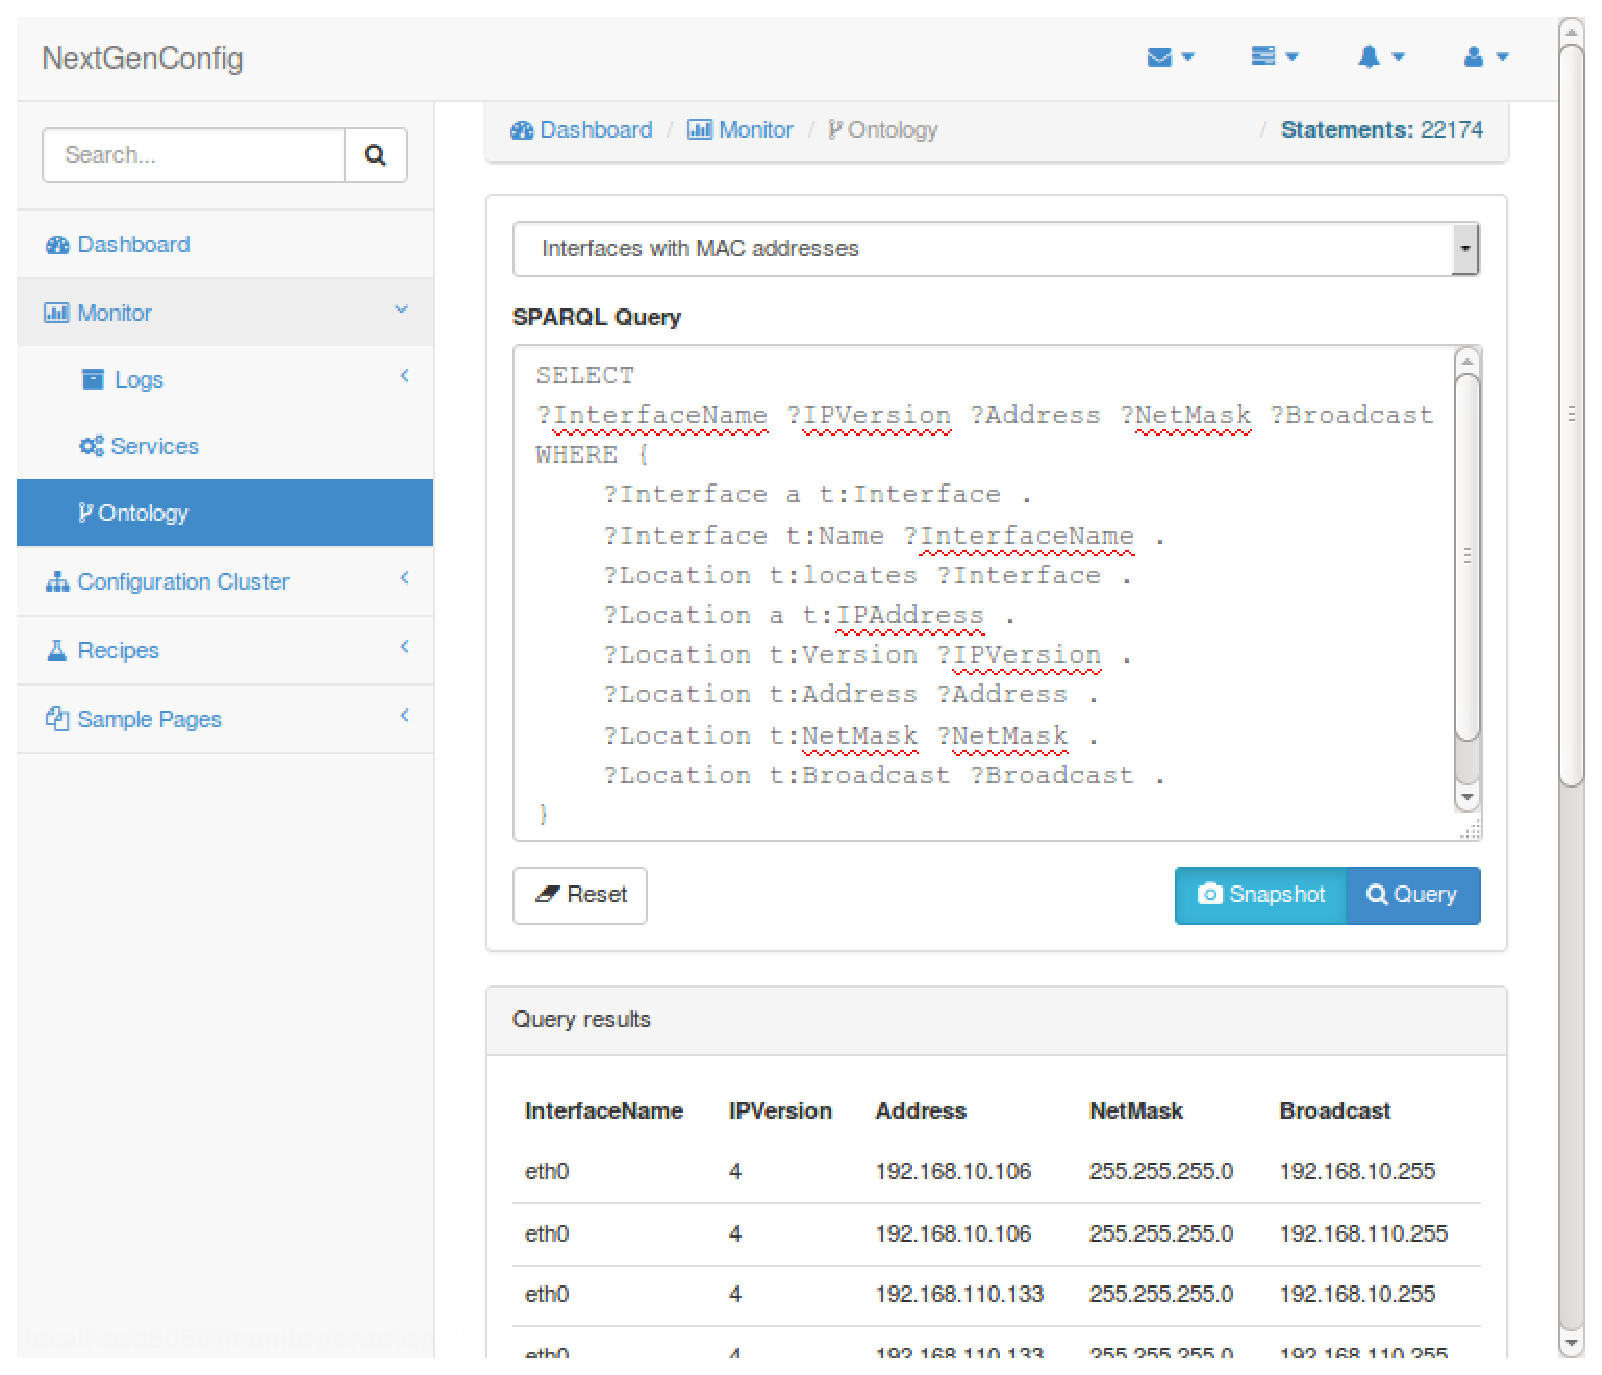
\includegraphics[width=\textwidth]{img/trifle_gui}}
    \caption{Interface d'administration du gestionnaire de configuration}
    \label{fig:trifle_gui}
\end{figure}


%%%%%%%%%%%%%%%%%%%%%%%%%%%%%%%%%%%%%%%%%%%%%%%%%%%%%%%%%%%%%%%%%%%%%%%

\chapter{Présentation d'EOLE}
\label{appendix:EOLE}

\section{Introduction}

Eole est un projet collaboratif basé sur la philosophie du logiciel libre.

La mutualisation des compétences et des moyens permet de réaliser des solutions
économiques, fiables et performantes.

\paragraph{EOLE} propose des solutions clef en main pour la mise en place de
serveurs Intranet/Internet.

Ces réalisations s’insèrent dans le cadre de réflexions et de recommandations
d’un certain nombre de structures et d’organismes ministériels favorables à
l’usage des logiciels libres dans l’administration.

\section{Modules EOLE}\label{modules eole}

Chaque module constitue une distribution GNU/LINUX spécifique qui permet
d’installer facilement un serveur dédié. Les services offerts sont
pré-configurés, l’ensemble est cohérent. Vous devez télécharger sur ce site
l’image ISO qui vous permettra de graver un DVD ou un CD d’installation. Ce
DVD/CD est multi module, le choix du module à installer est proposé au
démarrage (boot). 

\subsection{Amon}

Protéger les utilisateurs et les équipements.

Le pare feu Amon permet de partager en toute sécurité un accès Internet 
entre les sous réseaux d'un réseau local.

Installé sur un serveur dédié, équipé de deux, trois, quatre ou cinq 
interfaces réseau, il permet d'organiser au mieux votre réseau.
Des modèles de règles de pare feu sont disponibles pour chaque architecture.
Vous pouvez les utiliser tels quels ou bien les modifier à votre convenance. 
Un outil spécifique, Era, est à disposition pour effectuer ce travail.

\subsubsection{Principales fonctionnalités d'Amon}

\begin{itemize}
  \item Routage
  \item Support Vlan
  \item Authentification des utilisateurs
  \item Filtrage réseau
    \begin{itemize}
      \item Par IP (netfilter)
      \item par utilisateur (NuFW)
    \end{itemize}
  \item Filtrage de site amélioré
    \begin{itemize}
      \item Listes de sites interdits mises à jour quotidiennement
      \item Analyse sémantique des pages consultées
    \end{itemize}
  \item Réseau virtuel privé
  \item Suivi détaillé de la navigation web
  \item Mises à jour automatiques
  \item Journalisation des fichiers logs
  \item Détection d'intrusions
  \item Service de cache web
  \item Administration simplifiée
  \item Statistiques sur l'état du système
  \item Statistiques d'utilisation
\end{itemize}   

\subsection{Scribe}

Scribe est un contrôleur de domaine dotée de fonctions évoluées. 
Il optimise la gestion de votre parc de stations clientes.

Il dispose d'un annuaire qui référence, élèves, parents, personnels 
enseignant et administratifs, il propose un service de messagerie et héberge 
vos applications web au sein d'un portail Web 2.0

\subsubsection{Scribe est un contrôleur de domaine}

\begin{itemize}
  \item Gestion des connexions réseau des utilisateurs
  \item Partage de fichiers et de répertoires
  \item Support des ACL
  \item Partage d'imprimantes
  \item Gestion des comptes utilisateurs et des accès
  \item Gestion quotas disques et d'impression
  \item Exécution d'applications utilisateurs
\end{itemize}

\subsubsection{Scribe est un système de messagerie articulé autour d'un 
               annuaire performant}

\begin{itemize}
  \item L'annuaire est initialisé à partir d'importation de comptes 
        (SCONET, BE1D, AAF, CSV,...)
  \item L'annuaire peut servir de base d'authentification pour d'autres 
        services réseaux
  \item La messagerie gère deux domaines distincts (l'Internet et 
        l'intranet académique)
  \item Utilisation au choix d'une interface web multilingue ou d'un 
        client de messagerie standards
  \item Un service de listes de diffusion
  \item Une sécurité anti spam, un anti virus, une gestion de quotas 
        (taille des boites aux lettres)
\end{itemize}

\subsubsection{Scribe offre des services web => Envole 2.0}

\begin{itemize}
  \item Un serveur web
  \item Un portail web
  \item Des applications pré-installées
\end{itemize}

\subsubsection{Scribe est un serveur d'authentification unqiue (SSO)}

\begin{itemize}
  \item Eole SSO utilise l'annuaire LDAP
  \item Les standards C.A.S 2 et OpenID son supportés
  \item La fédération d'identité est possible via le protocole SAML
\end{itemize}

\subsubsection{Scribe dispose d'une gestion avancée des utilisateurs et 
               des postes clients}

\begin{itemize}
  \item Distribution de devoir
  \item Contrôle d'accès à Internet et au services réseaux
  \item Appliquer des restrictions ou pré configurer des applications, en
        fonction du login de l'utilisateur ou de ses groupes et du nom de 
        la machine sur laquelle il se connecte
  \item Effectuer des actions distantes sur les stations (fermer la 
        session, éteindre ou redémarrer un ou plusieurs postes)
  \item Surveiller la détection de virus par le serveur
\end{itemize}


\subsection{Horus}

Le module Horus est un contrôleur de domaine pour le réseau administratif 
d'un établissement scolaire ou d'un service académique.

Il offre toutes les fonctionnalités de partage de fichiers et d'imprimantes.

Il est également utilisable dans n'importe quelle autre structure 
nécessitant un contrôleur de domaine.

Un contrôleur de domaine est un serveur central qui est en charge des 
contrôles d'accès.

Un domaine est une entité logique qui reflète le plus souvent une 
organisation hiérarchique. Le domaine permet à l'administrateur système de 
gérer efficacement les utilisateurs des stations déployées car les 
informations (comptes et autorisations d'accès) sont centralisées dans une 
même base de données.

Le contrôleur de domaine permet donc :

\begin{itemize}
  \item De gérer des comptes utilisateur : ajouter, supprimer et modifier 
        un utilisateur
  \item De créer des groupes d'utilisateurs : créer des groupes pour 
        simplifier la gestion des politiques (permission sur des dossiers, 
        permission sur des services,...)
  \item De créer des politiques de sécurité qui seront appliquées aux 
        utilisateurs et aux groupes d'utilisateurs.
\end{itemize}            
 
L'utilisateur peut, sur une machine cliente raccordée au réseau, faire le 
choix de démarrer une session avec un compte du domaine ou avec un compte 
local s'il en existe. Il est ainsi possible d'ouvrir une session sur 
n'importe quel poste du domaine.

\subsection{Éclair}

Eclair est un serveur de clients légers linux.

Il permet de faire démarrer, depuis le réseau, des machines sans système
d'exploitation installé.

En pratique le serveur est la seule machine ayant un système installé, c'est 
lui qui exporte son système vers les clients légers. Tout ceci est 
complètement transparent pour l'utilisateur, il utilise le client léger, on 
dit aussi terminal, exactement comme s'il utilisait un ordinateur normal.

Tout le système et toutes les applications disponibles sur les terminaux étant
en fait installés sur le serveur, il n'y a qu'une seule machine à administrer.
Si vous installez une application sur le serveur, elle sera
immédiatement disponible pour tous les clients légers.

\subsection{Amon École}

Un seul serveur pour plusieurs modules.

Cela permet aux établissement d'avoir différents services sur une même machine
physique au lieu de multiplier le nombre de serveurs.

De ce fait, AmonEcole est particulière adapté aux petites structures en
termes d'effectif ou de moyens comme les écoles primaires ou les petits
collèges.

Il est également possible d'installer les module Horus (serveur de fichier)
et Eclair (clients légers)

En version 2.2 ces différents modules sont installés sur une seule machine
physique grâce à la technique de virtualisation (OpenVZ).

En version 2.3 on utilise le mode conteneur (LXC)

\subsection{Sphynx}

Le serveur Sphynx est un concentrateur de réseau virtuel privé.

Intégrant des composants logiciels de haute disponibilité, Sphynx vous permet
de relier en réseau vos serveurs pour former un réseau virtuel privé (RVP) 
avec le pare feu Amon dans les établissements distants et Sphynx en entrée de 
votre réseau.

Il fait parti des éléments constitutifs du réseau AGRIATES (Intranet Sécurisé
entre les Académie et les Etabissements scolaires).

\subsection{Zéphir}

Le module Zéphir propose une solution normalisée pour faciliter le
déploiement, la surveillance et la maintenance des modules EOLE.

Zéphir héberge une base de données des établissements et des serveurs 
installés dans ces établissements.

Zéphir permet la gestion de la configuration des serveurs

\begin{itemize}
  \item La génération des configurations serveurs (création du dictionnaire)
  \item Le stockage de ces configurations (fichier.eol)
  \item La distribution des ces configurations sur les serveurs via le réseau
  \item La mise à jour des configurations avec une gestion des différentes 
        versions et un historique des modifications effectuées
  \item Le lancement d'actions à distance
\end{itemize}

Zéphir dispose d'un module de surveillance de vos serveurs dans les 
établissements. Il permet la remontée d'alertes à intervalles réguliers. 
Des actions sur les serveurs en alerte peuvent être lancées automatiquement 
si besoin.


% ex: set spelllang=fr spell: %
%%% Local Variables: ***
%%% mode: latex ***
%%% TeX-master: "thesis.tex" ***
%%% End: ***


\end{spacing}
\end{document}

% ex: set spelllang=fr spell: %
%%% Local Variables: ***
%%% mode: latex ***
%%% TeX-master: "thesis.tex" ***
%%% End: ***
